%%%%%%%%%%%%%%%%%%%%%%%%%%%%%%%%%%%%%%%%%%%%%%%%%%%%%%%%%%%%%%%%%%%%%%%%%%%%%%%%
%2345678901234567890123456789012345678901234567890123456789012345678901234567890
%        1         2         3         4         5         6         7         8

%\documentclass[letterpaper, 10 pt, conference]{ieeeconf}  % Comment this line out if you need a4paper
\documentclass[a4paper, 10pt, conference]{ieeeconf}      % Use this line for a4 paper

\IEEEoverridecommandlockouts                              % This command is only needed if
                                                          % you want to use the \thanks command

\overrideIEEEmargins                                      % Needed to meet printer requirements.

\hyphenation{op-tical net-works semi-conduc-tor}

\usepackage{amsmath}
\usepackage{amsfonts}   % if you want the fonts
\usepackage{graphicx}
\usepackage{tikz}
\usepackage{scrextend}
%\linespread{0.95}
%\addtolength{\abovedisplayskip}{-1mm}
%\addtolength{\belowdisplayskip}{-1mm}
%\addtolength{\floatsep}{-1mm}
%\addtolength{\dbltextfloatsep}{-1mm}
%\addtolength{\intextsep}{-1mm}
%\addtolength{\dblfloatsep}{-1mm}
%\addtolength{\abovecaptionskip}{-5mm}
%\addtolength{\belowcaptionskip}{-15mm}
%\addtolength{\parskip}{-1mm}

\newcommand*\circled[1]{\tikz[baseline=(char.base)]{
            \node[shape=circle,draw,inner sep=0.5pt] (char) {#1};}}
\newcommand{\vect}[1]{\mbox{\boldmath${#1}$}}%$
\DeclareMathOperator*{\argmin}{arg\,min}
            


\title{Control of robots sharing their workspace with humans: an energetic approach to safety}
\author{Anis Meguenani$^{1}$, Vincent Padois$^{1}$ and Philippe Bidaud$^{1,2}$ 
\thanks{$^{1}$Anis Meguenani, Vincent Padois and Philippe Bidaud are with:}
\thanks{-Sorbonne Universit\'{e}, UPMC Univ Paris 06, UMR 7222, Institut des Syst\`{e}mes Intelligents et de Robotique, F-75005, Paris, France}
\thanks{-CNRS Centre National de la Recherche Scientifique, UMR 7222, Institut des Syst\`{e}mes Intelligents et de Robotique, F-75005, Paris, France}
\thanks{Email:{\tt\small \{meguenani,bidaud,padois\}@isir.upmc.fr}}
\thanks{$^{2}$Philippe Bidaud is with ONERA, 91123 Palaiseau, France}
\thanks{Email:{\tt\small philippe.bidaud@onera.fr}}}






\begin{document}

\maketitle

\begin{abstract}
For reactive control laws, input data for the operational task are usually discovered at every time-step. In this case, articular constraints such as joint limits are usually handled through inequalities. Depending on the expression of these constraints, compatibility issues can appear which can provoke constraints violation. Indeed coping with an articular position or velocity limit within a small amount of time (e.g. 1 \textit{ms}) may be impossible considering the limited reaction capabilities (i.e. deceleration and jerk) of the system. In this paper, we reformulate the articular position constraints to integrate the maximum deceleration in addition to the maximum jerk producible by the actuators. The joint rate constraint's expression is also modified to include jerk capabilities. The new formulations are implemented into a QP (quadratic programming) scheme to resolve the control problem of a redundant robot (KUKA LWR4) at the dynamic level. The resulting algorithm allows the automatic activation of the constraints, at the right time to comply with articular limits. A solution for the optimization control problem is guaranteed at every time-step and smoother control torques are produced.
\end{abstract}



% For peerreview papers, this IEEEtran command inserts a page break and
% creates the second title. It will be ignored for other modes.
\IEEEpeerreviewmaketitle



\section{Introduction}
\label{sec:intro constrcomp}

In practical applications, a control strategy for a robotic system is usually formulated depending on the nature of the operational task to be performed. Two kinds of strategies are distinguished : a proactive one when the objective of the operational task is already known (e. g. moving the end-effector from point A to point B) and a reactive strategy when the input data for the operational task are not known a priori but discovered at every time-step (e.g. tele-operation, co-manipulation applications...etc.). 

Independently from the control strategy, compliance to constraints and specifically to the physical constraints of the actuators is a must for any robotic system. This is particularly true in cases where constraints violation is highly critical (e.g. surgery, de-mining...etc.). 
\\
To ensure strict compliance, in case of a proactive control strategy, constraints and tasks can be handled offline. For example, to move the end-effector from point A to point B in the cartesian space, trajectories can be generated directly at the joint level. In this context, Katzschmann et. al in \cite{katzschmann2013towards} presented a trajectory generating algorithm that takes into account the actuators Max/min position, velocity, torque and even jerk capabilities. On the other hand, when tasks or constraints are not known in advance (reactive control case), \textit{trajectories cannot be generated} and it becomes impossible to use the same approach to cope with articular limitations. 


In the presented work, this issue is solved for robots controlled at the acceleration level. Constraints on the articular position, velocity, acceleration and jerk are expressed as inequality constraints within a QP formulation of the reactive control problem. The main contribution concerns the mathematical reformulation of the following constraints :

%\\
%For many critical applications including (surgery, de-mining, nuclear plant decommissioning,...), any robotic system must be able to cope with different constraints when achieving at best the operational tasks. In addition to the constraints induced by a static or dynamic environment, the applied control strategy should also take into account the actuators' limitations, i.e. articular positions, velocities, accelerations and jerk. In this paper, the focus is on the mathematical reformulation of the following constraints : 

\begin{itemize}
\item No violation of joint position bounds.
\item No violation of joint velocity bounds.
\end{itemize}
Within the new formulations, articular acceleration/deceleration and jerk capabilities are integrated to avoid incompatibilities. One kind of incompatibility can occur when inducing a braking phase to stop a motor's movement at a static\footnotetext[3]{We distinguish two types of bounds/constraints : \begin{itemize}
\item Static constraints : $x \leq x_{max}$ with : $x_{max}$ constant. 
\item Dynamic constraints : $x \leq \~{x}_{max}(t)$ with : $\~x_{max}(t)$ varying over time.
\end{itemize}
}
position constraint (i.e. Max/min allowed position) within a short period of time, for example one control time-step. This requires high deceleration and jerk capabilities that the robot may not be able to produce. Indeed, to be optimal, a robotic system must take the highest advantage of its dynamic capabilities within its limiting ranges. For example, to be as close as possible to an actuator's position limit with high articular acceleration and velocity and still be able to stop at time to not violate the constraint. This can be achieved through a braking phase triggered $n$ time-steps before reaching the limit and that takes into account the available deceleration capabilities, namely the torque and jerk. 
%The same idea can be extended to other static constraints and even dynamic ones.

In the case of redundant manipulators, the control problem can either be formulated at the kinematic level as the inversion of the following relation : 
\begin{equation}
\vect{\dot{X}} = J(\vect{q}) \dot{\vect{q}}
\label{eq:vel_kin_opt}
\end{equation}
or at the torque level when dynamic capabilities like contact forces control are needed : 
\begin{equation}
\vect{\ddot{X}} = \dot{J}(\vect{q}) \vect{\dot{q}} + J \ddot{\vect{q}}
\label{eq:X_ddot}
\end{equation}
$J(\vect{q})$, $\vect{\dot{X}}$, $\vect{\ddot{X}}$, $\vect{\dot{q}}$, $\vect{\ddot{q}}$ are respectively the operational task Jacobian matrix, the operational velocity and acceleration vectors and the joint velocity and acceleration vectors.
\\
When it is possible to implement constraints using an analytical scheme \cite{ngo2005passivity},\cite{ngo2006bounded}, the most general approach consists in formulating the control problem as a convex optimization one. Constraints are then expressed both through equalities and inequalities \cite{chen1994torque}-\cite{ma2002time}. The issue of constraints compatibility exists since a long time and remains an open one. In \cite{park1998enhanced} the problem of high peak of torques and chattering phenomena is highlighted when the joint angle limit of a serial robot is reached. This results from decelerating the limiting joint in order to stop the motion in one sampling time. the following problems appear :
\begin{enumerate}
\item Collision with the joint angle limit when no sufficient control torque nor jerk capabilities are available.
\item Vibration by exciting hidden resonant modes of the manipulator which can lead to instability.
\end{enumerate}
Park et al. in \cite{park1998enhanced} used a method called \textit{P-Step-Ahead Predictor (PSAP)}. The articular position and velocity limits are  detected far earlier and the braking phase is activated $p$ time-steps in advance to reduce the required amount of torque. In addition, the modulation of a weighting matrix related to the manipulability measure \cite{yoshikawa1985manipulability} is used for the same purpose. The problem with the proposed approach is the inevitable heuristic trial and error method to fix the acting parameters (e.g. $p$). Decré et al. in \cite{decre2009extending} were the first to  formulate a mathematical solution to directly integrate deceleration capabilities into the expression of a Cartesian position constraint; This resulted into a smoother articular velocity control input. Rubrecht et al. in \cite{rubrecht2010constraints} extended the idea to articular constraints. The deceleration capabilities  are integrated in the formulation of articular position constraints that are automatically activated $n$ time-steps before the joint position boundaries. Lange in \cite{lange2014predictive} and Suppa in \cite{lange2015trajectory} use a scaling method to generate an immediate Path-Accurate and Jerk-Limited stopping motion for industrial robots. This method can also be transposed and used when coping with articular limits. The correct time for triggering the stopping motion needs however to be computed. 
\\

The organization of this paper is as follows : In section II we study the relationship between the different actuation parameters $q$, $\dot{q}$, $\ddot{q}$ and the maximum allowed limits $[q_m, q_M]$, $[\dot{q}_m, \dot{q}_m]$, $[\ddot{q}_m, \ddot{q}_M]$, $[\dddot{q}_m, \dddot{q}_M]$ to expose the problem of articular constraints incompatibility.
Our main contribution is the introduction of the jerk limits in addition to the acceleration/deceleration capabilities for the expression of articular position and velocity  constraints : $(q_{m} \leq q \leq q_{M})$ and $(\dot{q}_{m} \leq \dot{q} \leq \dot{q}_{M})$. The braking phase is triggered automatically at the right moment to comply with the different constraints.
The obtained performances in simulation and experiments with a KUKA LWR4 are exposed and discussed in section III. Section IV is dedicated to conclusion and future work.



%%%%%%%%%%%%%%%%%%%%%%%%%%%%%%%%%%%%%%%%%%%%%%%%%%%%%%%%%
      %The QP form and Constraints Compatibility%
%%%%%%%%%%%%%%%%%%%%%%%%%%%%%%%%%%%%%%%%%%%%%%%%%%%%%%%%%

\section{The QP form and Constraints incompatibility cases}
This section aims at establishing the general formulation of the constrained, redundant inverse dynamic reactive control scheme. The objective is to compute the control torque $\boldsymbol{\tau}_{|k}^{c}$ in order to perform a trajectory tracking task while coping at every time-step with articular position, velocity, acceleration and jerk constraints. We highlight the fact that in this particular case the desired trajectory is \textit{discovered at every time-step} (tele-operation analogue situation) and not known in advance. Constraints incompatibility cases related to the classical way of expressing articular constraints are discussed. 


\subsection{Task formulation}

The objective function of the controller is defined as an error to be minimized. A cartesian acceleration task is considered and the error is between the expected acceleration $\vect{\ddot{X}}^c$ and the real acceleration $\vect{\ddot{X}}$ of the robot's end-effector. It is written in function of the control input $\vect{\tau}_{|k}^{c}$ :
\begin{equation}
 \vect{\ddot{X}}^{c} = J(\vect{q}) M(\vect{q})^{-1} \left(\boldsymbol{\tau}_{|k}^{c} - \vect{b}(\vect{q},\vect{\dot{q}})\right) + \dot{J}(\vect{q}) \vect{\dot{q}}
\label{Xddot}
\end{equation}
$\vect{b}(\vect{q},\vect{\dot{q}})$ are the non linear terms, namely gravity, Coriolis and centrifugal induced generalized forces. $M(\vect{q})$ is the joint space inertia matrix of the robot. $\vect{\ddot{X}}^c$ can be computed with a PD controller to track a desired trajectory (position $\vect{X}(t)^\star$ and velocity  $\vect{\dot{X}}(t)^\star$ discovered at every time-step. The acceleration task function to be minimized is written :
\hspace{-2mm}
\begin{equation}
\resizebox{.911\hsize}{!}{$\vect{g}\left(\boldsymbol{\tau}_{|k}^{c},\vect{\ddot{X}}^c\right) =  \vect{\ddot{X}}^c - \left(J(\vect{q}) M(\vect{q})^{-1} \left(\boldsymbol{\tau}_{|k}^{c} - \vect{b}(\vect{q},\vect{\dot{q}}) \right) + \dot{J}(\vect{q}) \vect{\dot{q}}\right)$}
\label{accelerationError}
\end{equation}





\subsection{Controller formulation}
The proposed control strategy computes the control torque by minimizing the norm of the  cartesian acceleration task function expressed in the following quadratic form : 
\begin{equation}
\argmin \limits_{\boldsymbol{\tau}_{|k}^{c}}  \left\| \vect{g}\left(\boldsymbol{\tau}_{|k}^{c},\vect{\ddot{X}}^c\right) \right\|_{Q_t}^2 + \epsilon  \| \boldsymbol{\tau}_{|k}^{c} \|_{Q_r}^2,
\label{eq:ctrl_pb}
\end{equation}
%subject to (\ref{eq:qddot_FINAL_CONSTR_1}) and (\ref{eq:qddot_FINAL_CONSTR_2}).
\\
$Q_t$ and $Q_r$ are  positive semidefinite weighting matrices and $\| \vect{a} \|_{Q}$ is the $Q-$weighted euclidean norm of $a$. $\epsilon  \| \boldsymbol{\tau} \|_{Q_r}^2$ with $\epsilon << 1$ serves as a regularization task in order to ensure the uniqueness of the control solution and to minimize the norm of the computed control torque. It can be shown that the quadratic forms composing the tasks can be written as functions of positive semidefinite matrices. This LQP optimization problem is therefore convex and admits a unique global solution. 
$\vect{\ddot{q}}_{|k}^{c}$ and $\vect{\tau}_{|k}^{c}$ are the control optimization variables : 
\begin{equation}
M(\vect{q}) \vect{\ddot{q}}_{|k}^{c} + \vect{b}(\vect{q},\vect{\dot{q}}) = \vect{\tau}_{|k}^{c}
\label{eq:dyn_eq}
\end{equation}
\\ 
In addition to the equality constraints corresponding to the dynamic equation \eqref{eq:dyn_eq}, the problem is also subject to inequality constraints described in the upcoming sections. 


\subsection{Articular constraints: classic formulation}
First, we introduce some notations that will be used throughout the paper :
\begin{itemize}
\item t $\in \mathbb{R}^{+}$ denotes time.
\item $k \in \mathbb{N}$ denotes the current discrete time-step.
\item $\delta t$ is the time-step duration of the discrete-time controller.
\item $\vect{q}_{|k}, \vect{\dot{q}}_{|k}, \vect{\ddot{q}}_{|k}, \vect{\dddot{q}}_{|k} \in \mathbb{R}$ are the joint position, velocity, acceleration and jerk at the current time-step $k$.
\item $\vect{q}_{M}, \vect{q}_{m}$ are the Max/min joint position boundaries.
\item $[\vect{\dot{q}}_{m}, \vect{\dot{q}}_{M}], [\vect{\ddot{q}}_{m}, \vect{\ddot{q}}_{M}], [\vect{\dddot{q}}_{m}, \vect{\dddot{q}}_{M}]}$ are the joint velocity, acceleration and jerk boundaries.
\end{itemize}
The computed control input $\boldsymbol{\tau}_{|k}^{c}$ at instant $k$ must be such that the articular limits are not violated at the next time-step $k+1$. These constraints can naturally be expressed in form of inequalities :
%\begin{equation} 
%\left\{\begin{array}{lcl}
%\vect{q}_{m} \leq \vect{q}_{|k+1} \leq \vect{q}_{M}, \\
%\vect{\dot{q}}_{m} \leq \vect{\dot{q}}_{|k+1} \leq \vect{\dot{q}}_{M}, \\
%\vect{\ddot{q}}_{m} \leq \vect{\ddot{q}}_{|k+1} \leq \vect{\ddot{q}}_{M}, \\
%%\boldsymbol{\tau}_{m} \leq \boldsymbol{\tau}_{|k} \leq \boldsymbol{\tau}_{M}.
%\vect{\dddot{q}}_{m} \leq \vect{\dddot{q}}_{|k+1} \leq \vect{\dddot{q}}_{M}, \\
%\end{array}\right.
%\label{eq:const_1}
%\end{equation}
\begin{equation} 
\left\{\begin{array}{lcl}
\begin{split}
\vect{q}_{m} & \leq \vect{q}_{|k+1} &\leq \vect{q}_{M},\\
\vect{\dot{q}}_{m} & \leq \vect{\dot{q}}_{|k+1} &\leq \vect{\dot{q}}_{M},\\
\vect{\ddot{q}}_{m} & \leq \vect{\ddot{q}}_{|k}^{c} &\leq \vect{\ddot{q}}_{M},\\
\boldsymbol{\tau}_{m} & \leq \boldsymbol{\tau}_{|k}^{c} &\leq \boldsymbol{\tau}_{M},\\
\vect{\dddot{q}}_{m}  & \leq \vect{\dddot{q}}_{|k+1} &\leq \vect{\dddot{q}}_{M}
\end{split}
\end{array}\right.
\label{eq:const_1_literature}
\end{equation}
$\boldsymbol{\ddot{q}}_m$, $\boldsymbol{\ddot{q}}_M$ can be computed as explained in Annexe A.
\\
To be easily accounted for, these constraints are expressed in function of the control variable $\vect{\ddot{q}}_{|k}^{c}$. Considering the literature \cite{rubrecht2010constraints}, \cite{decre2009extending}, the classic approach to do that is based on the system's state at instant $k$ and a local discrete linear approximation of its behaviour within a $\delta t$ time-step :  
\begin{equation} 
\left\{\begin{array}{l}
\begin{split}
\vect{q}_{|k+1} & = \vect{q}_{|k} + \delta t \vect{\dot{q}}_{|k} + \frac{\delta t^{2}}{2} \vect{\ddot{q}}_{|k},\\
\vect{\dot{q}}_{|k+1} &  =  \vect{\dot{q}}_{|k} + \delta t \vect{\ddot{q}}_{|k},\\
\vect{\dddot{q}}_{|k+1} &  =  \frac{1}{\delta t} (\vect{\ddot{q}}_{|k+1} - \vect{\ddot{q}}_{|k})
\end{split}
\end{array}\right.
\label{eq:Constr_1_time_step}
\end{equation}
Note : For a torque control input $\vect{\tau}_{|k}^{c}$ that is computed for the current time-step $k$ and equivalent to an acceleration command $\vect{\ddot{q}}_{|k}^{c}$ \eqref{eq:dyn_eq}, the expected articular acceleration at the next time-step $k+1$ can be written : 
\begin{equation} 
\vect{\ddot{q}}_{|k}^{c}  = \vect{\ddot{q}}_{|k+1} 
\label{eq:cmd_input_dyn}
\end{equation}
\\
Considering \eqref{eq:Constr_1_time_step}, constraints in \eqref{eq:const_1_literature} can be rewritten : 
\begin{equation} 
\resizebox{0.891\hsize}{!}{$
\left\{\begin{array}{l}
\begin{split}
%\vect{\ddot{q}}_{|k}^{c} \leq min(\frac{2(\vect{q}_{M}-\vect{q}_{|k}-\delta t \vect{\dot{q}}_{|k})}{\delta t^2}, \frac{(\vect{\dot{q}}_{M}-\vect{\dot{q}}_{|k})}{\delta t}, \vect{\ddot{q}}_{M}, \vect{\dddot{q}}_{M} \delta t+\vect{\ddot{q}}_{|k}),\\
%
%\vect{\ddot{q}}_{|k}^{c} \geq max(\frac{2(\vect{q}_{m}-\vect{q}_{|k}-\delta t \vect{\dot{q}}_{|k})}{\delta t^2}, \frac{(\vect{\dot{q}}_{m}-\vect{\dot{q}}_{|k})}{\delta t}, \vect{\ddot{q}}_{m}, \vect{\dddot{q}}_{m} \delta t+\vect{\ddot{q}}_{|k})
\frac{2}{\delta t^2} (\vect{q}_{m}-\vect{q}_{|k}-\delta t \vect{\dot{q}}_{|k}) \leq & \hspace{1.5mm} \vect{\ddot{q}}_{|k}^{c} \leq \frac{2}{\delta t^2} (\vect{q}_{M}-\vect{q}_{|k}-\delta t \vect{\dot{q}}_{|k}),\\
\frac{1}{\delta t} (\vect{\dot{q}}_{m}-\vect{\dot{q}}_{|k}) \leq  & \hspace{1.5mm} \vect{\ddot{q}}_{|k}^{c} \leq \frac{1}{\delta t} (\vect{\dot{q}}_{M}-\vect{\dot{q}}_{|k}),\\
\vect{\ddot{q}}_{m} \leq & \hspace{1.5mm} \vect{\ddot{q}}_{|k}^{c} \leq \vect{\ddot{q}}_{M},\\
\vect{\dddot{q}}_{m} \delta t+\vect{\ddot{q}}_{|k} \leq  & \hspace{1.5mm} \vect{\ddot{q}}_{|k}^{c} \leq \vect{\dddot{q}}_{M} \delta t+\vect{\ddot{q}}_{|k}
\end{split}
\end{array}\right.$}
\label{eq:Constr_time_step}
\end{equation}
When this classic formulation is used, the resulting constraints on the control variable $\vect{\ddot{q}}_{|k}^{c}$ are activated only one time-step before reaching the considered joint boundaries. In this situation, no sufficient braking time is available for the system and different incompatibility cases between the different constraints in (\ref{eq:Constr_time_step}) can appear. The optimization control problem becomes unsolvable. 
\subsubsection{Incompatibility cases related to joint rate limits}
Coping with a joint velocity constraint automatically imply bringing the articular acceleration $\vect{\ddot{q}}_{|k}$ to $0$ when hitting the Max/min velocity limit. In this case, a compatibility problem may arise if no sufficient articular jerk is producible by the actuators during the braking phase. Coping at the same time with joint rate limits and articular jerk limits may become impossible (see Fig.~\ref{fig:Constraints_incompatibility4}).

\subsubsection{Incompatibility cases related to joint position limits}
On the other hand, coping with joint position constraints imply bringing both articular velocity $\vect{\dot{q}}_{|k}$ and acceleration $\vect{\ddot{q}}_{|k}$ to $0$ when hitting the Max/min position boundaries. In this case, two compatibility problems may arise. The first is when no sufficient articular deceleration is available during the braking phase ($1$ control time-step). The second is when no sufficient jerk capabilities are available even if enough deceleration is producible by the actuators (see Fig.~\ref{fig:Constraints_incompatibility4}).
%
%For e.g. when the objective function of the QP requires an articular position beyond the actuation capabilities. No control torque nor jerk can be produced to brake and cope with the constraint (see Fig.~\ref{fig:Constraints_incompatibility4}).
%Three incompatibilities arise : 
%\begin{enumerate}
%\item Joint jerk and velocity limits.
%\item Joint acceleration and position limits. 
%\item Joint jerk and position limits. 
%\end{enumerate}
\begin{figure*}
\centering
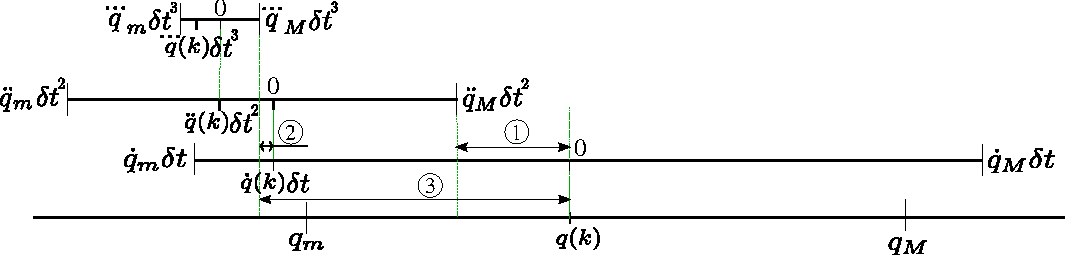
\includegraphics[width=2.0\columnwidth]{figures/Constraints_incompatibility4}
\caption{Constraints incompatibility one time step before $q_m$. No control acceleration $\ddot{q}_{|k}$ can be generated to make $\dot{q}_{|k+1} = 0$ by the next time step where $q_{|k+1}$ should be equal to $q_m$.}
\label{fig:Constraints_incompatibility4}
\end{figure*}

\section{Articular constraints: new formulation}
In this section, constraints incompatibility problems previously exposed are resolved. The formulation of joint velocity constraints is modified to include the system's jerk capabilities. Joint position constraints are also reformulated to take into account both the amounts of deceleration and jerk producible by the actuators.


\subsection{Joint velocity constraint incompatibility with jerk limits}
These constraints may become incompatible if a joint gets close to one of its velocity limits too fast (see Fig.~\ref{fig:Constraints_incompatibility4}). In this case, the admissible jerk may not be sufficient to allow a fast variation of the articular torque and it becomes impossible to bring the articular acceleration to zero within only one control time-step. The only solution to preserve compatibility is to jerk several time-steps before reaching the velocity boundary. The braking phase lasts therefore $(n_{1_{\mathbb{N}}} \geq 1)$ control time-steps. 
\\
Lets consider the braking phase for a joint hitting the maximum velocity limit $\vect{\dot{q}}_{M}$. The state of the system can be described as follows :
\begin{equation} 
\left\{\begin{array}{lcl}
\vect{\dot{q}}_{|k+1} = \vect{\dot{q}}_{|k} + \vect{\ddot{q}}_{|k} \delta t, \\
\vspace{2mm}
\vect{\ddot{q}}_{|k+1} = \vect{\ddot{q}}_{|k} + \vect{\dddot{q}}_{m} \delta t.
\end{array}\right.
\label{eq:discretized_dynamics_vel}
\end{equation}
with : $\vect{\dot{q}}_{|k} \geq 0$, $\vect{\ddot{q}}_{|k} \geq 0$ and  $\vect{\dddot{q}}_{m} \leq 0$ (braking phase). The joint velocity evolution in $n_1$ iterations is equal to the general form of the numerical sequence (\ref{eq:discretized_dynamics_vel}) :
\begin{equation}
\begin{split}
\vect{\dot{q}}_{|k+n_1} = \vect{\dot{q}}_{|k} + n_1 \vect{\ddot{q}}_{|k} \delta t + \frac{\delta t^2}{2} (n_1^2-n_1) \vect{\dddot{q}}_{m} 
\label{eq:q_dot_evolution_with_const_qdddot_m}
\end{split}
\end{equation}
Finally, in case of a dynamic-level control, the condition $\vect{\dot{q}}_{|k+n_1} \leq \vect{\dot{q}}_{M}$ for all integer $n_1$ leads to :
\begin{equation}
\begin{split}
\vect{\ddot{q}}_{|k}^{c} \leq \frac{(\vect{\dot{q}}_M-\vect{\dot{q}}_{|k})}{n_1 \delta t} - \frac{(n_1-1)}{2} \vect{\dddot{q}}_m \delta t 
\label{eq:q_ddot_vel_jerk_comp_aa_n1}
\end{split}
\end{equation}
$n_1$ is the integer minimizing the right hand side of (\ref{eq:q_ddot_vel_jerk_comp_aa_n1}). By diferentiating this expression w.r.t $n_1$ :
\begin{equation} 
\hspace{-4mm}
\left. \begin{array}{r} 
n_1 \geq 1 \\
\frac{-(\vect{\dot{q}}_M-\vect{\dot{q}}_{|k})}{n_1^2 \delta t} - \frac{\delta t}{2} \vect{\dddot{q}}_m  = 0
\end{array} \right\} 
\Rightarrow n_1=-\frac{\sqrt{-2\vect{\dddot{q}}_m(\vect{\dot{q}_M}-\vect{\dot{q}}_{|k})}}{\vect{\dddot{q}}_m \delta t}
\label{eq:n_1_eq_aa}
\end{equation}
Following the same method for the lower velocity constraint, the condition $\vect{\dot{q}}_{|k+n_2} \geq \vect{\dot{q}}_{m}$ for all integer $n_2 \geq 1$ becomes : 
\begin{equation}
\begin{split}
\vect{\ddot{q}}_{|k}^{c} \geq \frac{(\vect{\dot{q}}_m-\vect{\dot{q}}_{|k})}{n_1 \delta t} - \frac{(n_2-1)}{2} \vect{\dddot{q}}_M \delta t
\label{eq:q_ddot_vel_jerk_comp_aa_n2}
\end{split}
\end{equation}
With :
\begin{equation}
n_2 = -\frac{\sqrt{-2\vect{\dddot{q}}_M(\vect{\dot{q}_m}-\vect{\dot{q}}_{|k})}}{\vect{\dddot{q}}_M \delta t} 
\label{eq:n_2_eq_aa}
\end{equation}
Maximizing the right hand side of (\ref{eq:q_ddot_vel_jerk_comp_aa_n2}).
The reflected constraint on the control variable $\vect{\ddot{q}}_{|k}^{c}$ is of the form : 
\begin{equation}
\begin{split}
f_2(\vect{\dot{q}}_m, \vect{\dddot{q}}_M) \leq \vect{\ddot{q}}_{|k}^{c} \leq f_1(\vect{\dot{q}}_M, \vect{\dddot{q}}_m) 
\label{eq:qddot_cond_to_satisfy_Jerk_Vel_compatibility_profile}
\end{split}
\end{equation}
$f_1$ and $f_2$ are as in (\ref{eq:q_ddot_vel_jerk_comp_aa_n1}) and (\ref{eq:q_ddot_vel_jerk_comp_aa_n2}).



\subsection{Joint position constraint incompatibility with deceleration and/or jerk limits}
These constraints may become incompatible if a joint gets close to one of its position limits too fast (see Fig.~\ref{fig:Constraints_incompatibility4}). In this case, the admissible deceleration and/or jerk may not be sufficient to allow a fast variation of the articular torque and it becomes impossible to bring both articular acceleration and velocity to zero within only one time-step. For example, the braking phase to cope with an upper position limit is as follows : the concerned actuator starts jerking with maximum capability in the opposite direction. If the maximum producible deceleration is reached, braking jerk is then equal to zero and this maximum deceleration is used to stop the joint at the position boundary. By the end, deceleration is also brought back to zero. As explained before, coping with a joint's position constraint may fail because of incompatibilities with two other constraints : articular deceleration limits and jerk limits (\ref{eq:const_1_literature}). The resolution of these incompatibilities will be performed as following. First, the expression of position constraints in (\ref{eq:Constr_time_step}) is modified to include deceleration capabilities ($\vect{\ddot{q}}_m$ and $\vect{\ddot{q}}_M$) that will be used for $n_{3_{\mathbb{N}}$ time-steps during the braking phase to cope with the Max/min allowed positions. In this case, jerk capabilities are not considered. The reflected constraints on the control variable $\vect{\ddot{q}_{|k}^{c}}$ will be of the form : 
\begin{equation}
\begin{split}
f_3(\vect{q}_m, \vect{\ddot{q}}_M) \leq \vect{\ddot{q}}_{|k}^{c} \leq f_4(\vect{q}_M, \vect{\ddot{q}}_m) 
\label{eq:qddot_cond_to_satisfy_Acc_posi_compatibility}
\end{split}
\end{equation}
Secondly, the expression in (\ref{eq:Constr_time_step}) is also modified to include jerk capabilities ($\vect{\dddot{q}}_m$ and $\vect{\dddot{q}}_M$) that will be used for $n_{5_{\mathbb{N}}$ time-steps during the braking phase. Independently from deceleration capabilities. The reflected constraints on the control variable  is of the form :
\begin{equation}
\begin{split}
f_5(\vect{q}_m, \vect{\dddot{q}}_M) \leq \vect{\ddot{q}}_{|k}^{c} \leq f_6(\vect{q}_M, \vect{\dddot{q}}_m) 
\label{eq:qddot_cond_to_satisfy_Jerk_posi_compatibility}
\end{split}
\end{equation}
Finally, based on these two new formulations, an expression of the position constraint that takes into account at the same time both deceleration and braking jerk capabilities is formulated. The reflected constraints on the control variable $\vect{\ddot{q}}_{|k}^{c}$ will be of the form : 
\begin{equation}
\begin{split}
f_7(\vect{q}_m, \vect{\ddot{q}}_M, \vect{\dddot{q}}_M) \leq \vect{\ddot{q}}_{|k}^{c} \leq f_8(\vect{q}_M, \vect{\ddot{q}}_m, \vect{\dddot{q}}_m) 
\label{eq:qddot_cond_to_satisfy_Acc_Jerk_posi_compatibility}
\end{split}
\end{equation}
$f_3$, $f_4$, $f_5$, $f_6$, $f_7$, $f_8$ will be defined as follows. 
\\
\subsubsection{Joint position constraint incompatibility with deceleration limits}
We consider the braking phase for a joint hitting the upper position bound $\vect{q}_{M}$. In this case, the maximum producible deceleration is $\vect{\ddot{q}}_{m}$. Jerk capabilities $\vect{\dddot{q}}_{m}$ are considered infinite. The state of the system during this phase can be described by :
\begin{equation} 
\left\{\begin{array}{lcl}
\vect{q}_{|k+1} = \vect{q}_{|k} + \vect{\dot{q}}_{|k} \delta t, \\
\vspace{2mm}
\vect{\dot{q}}_{|k+1} = \vect{\dot{q}}_{|k} + \vect{\ddot{q}}_{m} \delta t.
\end{array}\right.
\label{eq:discretized_dynamics_posi_decel}
\end{equation}
with : $\vect{q}_{|k} \geq 0$, $\vect{\dot{q}}_{|k} \geq 0$ and  $\vect{\ddot{q}}_{m} \leq 0$ (braking phase). The joint position evolution in $n_3  \geq 1$ iterations is equal to the general form of the numerical sequence (\ref{eq:discretized_dynamics_posi_decel}) :
\begin{equation}
\begin{split}
\vect{q}_{|k+n_3} = \vect{q}_{|k} + n_3 \vect{\dot{q}}_{|k} \delta t + \frac{\delta t^2}{2} (n_3^2-n_3) \vect{\ddot{q}}_{m} 
\label{eq:q_evolution_with_const_qddot_m}
\end{split}
\end{equation}
Finally the condition $\vect{q}_{|k+n_3} \leq \vect{q}_{M}$ for all integer $n_3$ leads to :
\begin{equation}
\begin{split}
\vect{\dot{q}}_{|k}^{c} \leq \frac{(\vect{q}_M-\vect{q}_{|k})}{n_3 \delta t} - \frac{(n_3-1)}{2} \vect{\ddot{q}}_m \delta t
\label{eq:q_dot_posi_acc_comp}
\end{split}
\end{equation}
$\vect{\dot{q}}_{|k}^{c}$ is the velocity control input in case the robot is controlled at the kinematic level. According to Annex A, the equivalent constraint on the acceleration control variable $\vect{\ddot{q}}_{|k}^{c}$ in case the robot is controlled at the dynamic level (our case) and that generates the same braking phase is written :
\begin{equation}
\begin{split}
\vect{\ddot{q}}_{|k}^{c} \leq \frac{(\vect{q}_M-\vect{q}_{|k})}{n_3 \delta t^2} - \frac{\vect{\dot{q}}_{|k}}{\delta t} - \frac{(n_3-1)}{2} \vect{\ddot{q}}_m 
\label{eq:q_ddot_posi_acc_comp_upp}
\end{split}
\end{equation}
With : 
\begin{equation}
\begin{split}
n_3 = \frac{-\sqrt{-2 \vect{\ddot{q}}_m (\vect{q}_M - \vect{q}_{|k})}}{\vect{\ddot{q}}_m \delta t}
\label{eq:n_3_Acc_posi_comp}
\end{split}
\end{equation}
The integer minimizing the right-hand side of (\ref{eq:q_ddot_posi_acc_comp_upp}).
\\
Following the same reasoning for the lower position limit, the condition $\vect{q}_{|k+n_4} \geq \vect{q}_{m}$ for all integer $n_4 \geq 1$ becomes :
\begin{equation}
\begin{split}
\vect{\ddot{q}}_{|k}^{c} \geq \frac{(\vect{q}_m-\vect{q}_{|k})}{n_4 \delta t^2} - \frac{\vect{\dot{q}}_{|k}}{\delta t} - \frac{(n_4-1)}{2} \vect{\ddot{q}}_M 
\label{eq:q_ddot_posi_acc_comp_low}
\end{split}
\end{equation}
With : 
\begin{equation}
\begin{split}
n_4 = \frac{\sqrt{-2 \vect{\ddot{q}}_M (\vect{q}_m - \vect{q}_{|k})}}{\vect{\ddot{q}}_M \delta t}
\label{eq:n_4_Acc_posi_comp}
\end{split}
\end{equation}
Maximizing the right hand side of (\ref{eq:q_ddot_posi_acc_comp_low})
%\\
%Independently from jerk ($\dddot{q}_m$ and $\dddot{q}_M$ infinite) and as described in \cite{rubrecht2010constraints}, these two constraints become incompatible if an actuator gets close to one of its position limits with a high acceleration (cf \ref{fig:Constraints_incompatibility4}) : the producible deceleration (between $\ddot{q}_m$ and $\ddot{q}_M$) may not be sufficient to make $\dot{q}_{|k+1}=0$ at $q_{|k+1} = q_m$. The only way to preserve compatibility is to decelerate several time steps before the position limit. As shown in Annexe A, ensuring :
%
%%
%%\begin{equation}
%%\begin{split}
%%q(k+n_3) = q_{|k} + n_3 \dot{q}_{|k} \delta t + \frac{1}{2} (n_3^2 - n_3) \dddot{q}_m_{|k} \delta t^2 < q_M
%%\label{eq:Constr_on_Fc1_3}
%%\end{split}
%%\end{equation}
%%
%%\begin{equation}
%%\begin{split}
%%q(k+n_4) = q_{|k} + n_4 \dot{q}_{|k} \delta t + \frac{1}{2} (n_4^2 - n_4) \dddot{q}_m_{|k} \delta t^2 < q_M
%%\label{eq:Constr_on_Fc1_4}
%%\end{split}
%%\end{equation}
%%
%%Which can be written :
%%
%\begin{equation}
%\begin{split}
%\ddot{q}_{|k}  \leq  \frac{2(q_M - q_{|k+1})}{n_3 \delta t^2} - \frac{(n_3-1) \ddot{q}_m}{2} - \frac{\dot{q}_{|k}}{\delta t}
%\label{eq:qddot_cond_to_satisfy_Acc_posi_compatibility_1}
%\end{split}
%\end{equation}
%
%\begin{equation}
%\begin{split}
%\ddot{q}_{|k} \geq \frac{2(q_m - q_{|k+1})}{n_4 \delta t^2} - \frac{(n_4-1) \ddot{q}_M}{2} - \frac{\dot{q}_{|k}}{\delta t}  
%\label{eq:qddot_cond_to_satisfy_Acc_posi_compatibility_2}
%\end{split}
%\end{equation}
%
%
%With :
%
%\begin{equation}
%\begin{split}
%n_3 = \frac{-\sqrt{-2 \ddot{q}_m (q_M - q_{|k})}}{\ddot{q}_m \delta t}
%\label{eq:n_1_Acc_posi_comp}
%\end{split}
%\end{equation}
%
%
%
%\begin{equation}
%\begin{split}
%n_4 = \frac{\sqrt{-2 \ddot{q}_M (q_m - q_{|k})}}{\ddot{q}_M \delta t}
%\label{eq:n_2_Acc_posi_comp}
%\end{split}
%\end{equation}
%
%enables to decelerate the joint so that both position limit and maximum deceleration capabilities are satisfied. The resulting constraint on $\ddot{q}$ has the following profile : 
%
%
%\begin{equation}
%\begin{split}
%f_3(q_m, \ddot{q}_M) \leq \ddot{q}_{|k} \leq f_4(q_M, \ddot{q}_m) 
%\label{eq:qddot_cond_to_satisfy_Acc_posi_compatibility}
%\end{split}
%\end{equation}
%
%In this case, only the deceleration capabilities are considered for coping with the position limits. However, in reality, jerk limitations are also to be considered. 
\subsubsection{Joint position constraint incompatibility with jerk limits}
As already explained, in this case only maximum jerk capabilities are considered during the braking phase to cope with position constraints. Deceleration capabilities are considered infinite. For an upper position bound $\vect{q}_M$, $\vect{\dddot{q}}_m$ the maximum braking jerk; The state of the system during the braking phase can be described as : 
\begin{equation} 
\left\{\begin{array}{lcl}
\vect{q}_{|k+1} = \vect{q}_{|k} + \vect{\dot{q}}_{|k} \delta t, \\
\vspace{2mm}
\vect{\dot{q}}_{|k+1} = \vect{\dot{q}}_{|k} + \vect{\ddot{q}} \delta t, \\
\vect{\ddot{q}}_{|k+1} = \vect{\ddot{q}}_{|k} + \vect{\dddot{q}}_{m} \delta t
\end{array}\right.
\label{eq:discretized_dynamics_posi_jerk_braking}
\end{equation}
with : $\vect{q}_{|k} \geq 0$, $\vect{\dot{q}}_{|k} \geq 0$ and  $\vect{\dddot{q}}_{m} \leq 0$. The joint position evolution in $n_5$ iterations is equal to the general form of the numerical sequence (\ref{eq:discretized_dynamics_posi_jerk_braking}) :
\begin{equation}
\begin{split}
\vect{q}_{|k+n_5} = \vect{q}_{|k} + n_5 \vect{\dot{q}}_{|k} \delta t & +  \frac{(n_5^2-n_5)}{2} \vect{\ddot{q}}_{|k} \delta t^2 \\
& + (\frac{n_5^3}{6}-\frac{n_5^2}{2}+\frac{n_5}{3}) \vect{\dddot{q}}_m \delta t^3
\label{eq:q_evolution_with_const_qdddot_m}
\end{split}
\end{equation}
Finally the condition $\vect{q}_{|k+n_5} \leq \vect{q}_{M}$ for all integer $n_5$ leads to :
\begin{equation}
\begin{split}
\vect{\ddot{q}}_{|k}^{c} \leq \frac{2(\vect{q}_M-\vect{q}_{|k})}{(n_5^2-n_5) \delta t^2} - \frac{2 \vect{\dot{q}}_{|k}}{(n_5-1) \delta t} - \frac{(\frac{n_5^2}{3}-n_5+\frac{2}{3})}{(n_5-1)}\vect{\dddot{q}}_m \delta t
\label{eq:q_ddot_posi_jerk_comp_upp}
\end{split}
\end{equation}
$n_5$ is the integer minimizing the right hand side of (\ref{eq:q_ddot_posi_jerk_comp_upp}); It can be computed analytically or numerically. By differentiating this expression w.r.t $n_5$ :
\begin{equation}
\left\{\begin{array}{lcl}
n_5 \geq 3, \\
\begin{split}
-&(\frac{1}{3} \vect{\dddot{q}}_m \delta t^3) n_5^4 + (\frac{2}{3} \vect{\dddot{q}}_{|m} \delta t^3) n_5^3  \\
+&(2 \vect{\dot{q}}_{|k} \delta t - \frac{1}{3} \vect{\dddot{q}}_m \delta t^3) n_5^2 \\
+& 4 (\vect{q}_M-\vect{q}_{|k}) n_5 - 2(\vect{q}_M-\vect{q}_{|k})=0
\end{split}
\end{array}\right.
\label{eq:n_5_eq_new}
\end{equation}
$n_5$ is the rounded up real root of (\ref{eq:n_5_eq_new}) that minimizes (\ref{eq:q_ddot_posi_jerk_comp_upp}). $n_5$ must be $\geq 3$ so $\vect{\dddot{q}}_m$ is always part of (\ref{eq:q_ddot_posi_jerk_comp_upp}). 
\\
Following the same reasoning for the lower position limit, when reflected on the acceleration control parameter, the condition $\vect{q}_{|k+n_6} \geq \vect{q}_{m}$ for all integer $n_6 \geq 3$ can be expressed :
\begin{equation}
\begin{split}
\vect{\ddot{q}}_{|k}^{c}  \geq \frac{2(\vect{q}_m - \vect{q}_{|k})}{(n_6^2 - n_6)\delta t^2} - \frac{2 \vect{\dot{q}}_{|k}}{(n_6-1)\delta t} 
- \frac{(\frac{n_6^2}{3} - n_6 + \frac{2}{3})}{(n_6-1)}\vect{\dddot{q}}_M_{|k} \delta t
\label{eq:q_ddot_posi_jerk_comp_low}
\end{split}
\end{equation}
With : 
\begin{equation}
\left\{\begin{array}{lcl}
n_6 \geq 3, \\
\begin{split}
-&(\frac{1}{3} \vect{\dddot{q}}_M \delta t^3) n_6^4 + (\frac{2}{3} \vect{\dddot{q}}_{|M} \delta t^3) n_6^3  \\
+&(2 \vect{\dot{q}}_{|k} \delta t - \frac{1}{3} \vect{\dddot{q}}_M \delta t^3) n_6^2 \\
+& 4 (\vect{q}_m-\vect{q}_{|k}) n_6 - 2(\vect{q}_m-\vect{q}_{|k})=0
\end{split}
\end{array}\right.
\label{eq:n_6_eq_new}
\end{equation}
$n_6$ is the rounded up real root of (\ref{eq:n_6_eq_new}) that maximizes the right hand side of (\ref{eq:q_ddot_posi_jerk_comp_low}).
%Independently from acceleration capabilities (infinite $\ddot{q}_m$ and $\ddot{q}_M$), no jerk (between $\dddot{q}_m$ and $\dddot{q}_M$) can be generated to allow the deployment of an acceleration that will make $\dot{q}_{|k+1}=0$ at $q_{|k+1} = q_m$. As shown in Annexe A, ensuring :
%
%
%%\begin{equation}
%%\begin{split}
%%q(k+n_5) = q_{|k} + n_5 \dot{q}_{|k} \delta t + \frac{n_5^2 - n_5}{2} \ddot{q}_{|k} \delta t^2 & + \\
%%(\frac{n_5^3}{6} - \frac{n_5^2}{2} + \frac{n_5}{3}) \dddot{q}_m_{|k} \delta t^3 < q_M
%%\label{eq:Constr_on_Fc1_1}
%%\end{split}
%%\end{equation}
%%
%%\begin{equation}
%%\begin{split}
%%q(k+n_6) = q_{|k} + n_6 \dot{q}_{|k} \delta t + \frac{n_6^2 - n_6}{2} \ddot{q}_{|k} \delta t^2 & + \\
%%(\frac{n_6^3}{6} - \frac{n_6^2}{2} + \frac{n_6}{3}) \dddot{q}_M_{|k} \delta t^3 > q_m
%%\label{eq:Constr_on_Fc1_2}
%%\end{split}
%%\end{equation}
%%
%%Which can be written : 
%\begin{equation}
%\begin{split}
%\ddot{q}_{|k} \leq \frac{2(q_M - qk))}{(n_5^2 - n_5)\delta t^2} & - \frac{2 \dot{q}_{|k}}{(n_5-1)\delta t} \\
%& - \frac{(\frac{n_5^2}{3} - n_5 + \frac{2}{3} \dddot{q}_m_{|k} \delta t^2)}{(n_5-1)}
%\label{eq:qddot_cond_to_satisfy_compatibility_1}
%\end{split}
%\end{equation}
%
%\begin{equation}
%\begin{split}
%\ddot{q}_{|k}  \geq \frac{2(q_m - q_{|k})}{(n_6^2 - n_6)\delta t^2} & - \frac{2 \dot{q}_{|k}}{(n_6-1)\delta t} \\
%& - \frac{(\frac{n_6^2}{3} - n_6 + \frac{2}{3} \dddot{q}_M_{|k} \delta t^2)}{(n_6-1)}
%\label{eq:qddot_cond_to_satisfy_compatibility_2}
%\end{split}
%\end{equation}
%
%With $n_5, n_6$ respectively chosen to minimize the right hand side of (\ref{eq:qddot_cond_to_satisfy_compatibility_1}) and (\ref{eq:qddot_cond_to_satisfy_compatibility_2}).
%
%%$n_5$ and $n_6$ are the closest integers to the real roots of the following polynomials of degree $4$ : 
%%
%%
%%\begin{equation}
%%\begin{split}
%%(-\frac{\dddot{q}_m_{|k} \delta t^3}{3}) n_5^4 + (2 \frac{\dddot{q}_m_{|k} \delta t^3}{2}) n_5^3 + \\ (\frac{\dddot{q}_m_{|k} \delta t^6 + 6 \dot{q}_{|k} \delta t^4}{3}) n_5^2 + \\(4 (q_M - q_{|k})) n_5 - (2 (q_M - q_{|k}))
%%\label{eq:polynom_4_1}
%%\end{split}
%%\end{equation}
%%
%%
%%\begin{equation}
%%\begin{split}
%%(-\frac{\dddot{q}_M_{|k} \delta t^3}{3}) n_6^4 + (2 \frac{\dddot{q}_M_{|k} \delta t^3}{2}) n_6^3 + \\ (\frac{\dddot{q}_M_{|k} \delta t^6 + 6 \dot{q}_{|k} \delta t^4}{3}) n_6^2 + \\(4 (q_m - q_{|k})) n_6 - (2 (q_m - q_{|k}))
%%\label{eq:polynom_4_2}
%%\end{split}
%%\end{equation}
%
%enables to decelerate the joint so that maximal jerk and joint position limits are both satisfied. The resulting constraint on $\ddot{q}$ has the following profile : 
%
%\begin{equation}
%\begin{split}
%f_5(q_m, \dddot{q}_M) \leq \ddot{q}_{|k} \leq f_6(q_M, \dddot{q}_m) 
%\label{eq:qddot_cond_to_satisfy_Acc_posi_compatibility}
%\end{split}
%\end{equation}
\subsubsection{Joint position constraint with both deceleration and jerk limits}
As explained before, both joint deceleration ($\vect{\ddot{q}_m}, \vect{\ddot{q}_M}$) and braking jerk capabilities ($\vect{\dddot{q}_m}, \vect{\dddot{q}_M}$) should be part of the new formulation of articular position constraints. The resulting constraint on the acceleration control variable (\ref{eq:qddot_cond_to_satisfy_Acc_Jerk_posi_compatibility}) will enforce a braking phase at the right time to cope with position limits considering the reaction capabilities of the actuators. As said before, to cope with position constraints, the considered actuator starts jerking in the opposite direction until maximum deceleration is reached, this deceleration is then used to stop the joint's movement at the position's boundary. For an upper position limit $\vect{q}_{M}$, Based on (\ref{eq:q_evolution_with_const_qddot_m}), the position's evolution during the braking phase in $n_{7_{\mathbb{N}}}+n_{9_{\mathbb{N}}}$ iterations can be expressed : 
\begin{equation}
\begin{split}
\vect{q}_{|k+n_7+n_9}=\vect{q}_{|k+n_7} + n_9 \vect{\dot{q}}_{|k+n_7} \delta t + \frac{(n_9^2-n_9)}{2} \vect{\ddot{q}}_m \delta t^2
\label{eq:q_evolution_with_const_qddot_m_and_qdddot_m_final}
\end{split}
\end{equation} 
$\vect{q}_{|k+n_7}$ and $\vect{\dot{q}}_{k+n_7}$ respectively equivalent to (\ref{eq:q_evolution_with_const_qdddot_m}) and   (\ref{eq:q_dot_evolution_with_const_qdddot_m}). When developed,
(\ref{eq:q_evolution_with_const_qddot_m_and_qdddot_m_final}) can be written : 
\begin{equation}
\begin{split}
\vect{q}_{|k+n_7+n_9} = \vect{q}_{|k} & + (n_7+n_9) \vect{\dot{q}}_{|k} \delta t \\
                      & + (\frac{n_7^2-n_7}{2}+n_7 n_9) \vect{\ddot{q}}_{|k} \delta t^2 \\
                      & + \frac{(n_9^2-n_9)}{2} \vect{\ddot{q}}_m \delta t^2\\
                      & + [\frac{n_7^3}{6}-\frac{n_7^2}{2}+\frac{n_7}{3}+\frac{n_9(n_7^2-n_7)}  {2}] \vect{\dddot{q}}_m \delta t^3 
                      
\label{eq:q_evolution_with_const_qddot_m_and_qdddot_m_2_final}
\end{split}
\end{equation} 
with : $\vect{q}_{|k} \geq 0$, $\vect{\dot{q}}_{|k} \geq 0$ , $\vect{\ddot{q}}_m \leq 0$ and $\vect{\dddot{q}}_m \leq 0$ (braking phase). The condition $\vect{q}_{|k+n_7+n_9} \leq \vect{q}_M$ for all integers ($n_7$, $n_9$) in case of a dynamic level control can be expressed :
\begin{equation}
\begin{split}
\vect{\ddot{q}}_{|k}^{c} & \leq \frac{(\vect{q}_M - \vect{q}_{|k})}{(\frac{n_7^2 - n_7}{2} + n_7 n_9)\delta t^2} - \frac{(n_7+n_9)}{(\frac{n_7^2 - n_7}{2} + n_7 n_9) \delta t} \vect{\dot{q}}_{|k}\\
& - \frac{(n_9^2-n_9)}{(n_7^2 - n_7 + 2 n_7 n_9)}  \vect{\ddot{q}}_m \\
& -\frac{[\frac{n_7^3}{6} - \frac{n_7^2}{2} + \frac{n_7}{3} + \frac{n_9(n_7^2-n_7)}{2}]}{(\frac{n_7^2 - n_7}{2} + n_7 n_9)} \vect{\dddot{q}}_m \delta t 
\label{eq:Constr_comp_posi_acc_jerk_1_final}
\end{split}
\end{equation}
In case the control is performed at the kinetic level, the constraint is reflected on $\vect{\dot{q}}_{|k}^{c}$ : 
\begin{equation}
\begin{split}
\vect{\dot{q}}_{|k}^{c} & \leq \frac{(\vect{q}_M - \vect{q}_{|k})}{(n_7 + n_9) \delta t}  -\frac{[\frac{(n_7^2-n_7)}{2} + n_7 n_9]}{(n_7 + n_9)}  \vect{\ddot{q}}_{|k} \delta t\\ 
 & - \frac{(n_9^2-n_9)}{2(n_7 + n_9)} \vect{\ddot{q}}_m \delta t \\
           & - \frac{[\frac{(n_7^3)}{6} + \frac{(n_7^2)}{2} + \frac{(n_7)}{3} + \frac{n_9 (n_7^2 - n_7)}{2}]}{(n_7 + n_9)} \vect{\dddot{q}}_m \delta t^2 
\label{eq:Constr_comp_posi_acc_jerk_1_kinema_final}
\end{split}
\end{equation}
Computed numerically, ($n_7$, $n_9$) are two integers minimizing the right hand side of (\ref{eq:Constr_comp_posi_acc_jerk_1_final}). $n_7 \geq 1$ and $n_9 \geq 3$.
Following the same reasoning for the lower position limit, the constraint $\vect{q}_{|k+n_8+n_{10}} \geq \vect{q}_m$ for all integers ($n_8 \geq 1$, $n_{10} \geq 3$), when reflected on the acceleration control variable can be expressed : 
\begin{equation}
\begin{split}
\vect{\ddot{q}}_{|k}^{c} & \geq \frac{(\vect{q}_m - \vect{q}_{|k})}{(\frac{n_8^2 - n_8}{2} + n_8 n_{10})\delta t^2} \\ 
                     & - \frac{(n_8+n_{10})}{(\frac{n_8^2 - n_8}{2} + n_8 n_{10}) \delta t} \vect{\dot{q}}_{|k} - \frac{(n_{10}^2-n_{10})}{(n_8^2 - n_8 + 2 n_8 n_{10})}  \vect{\ddot{q}}_M \\
                     & -\frac{[\frac{n_8^3}{6} - \frac{n_8^2}{2} + \frac{n_8}{3} + \frac{n_{10}(n_8^2-n_8)}{2}]}{(\frac{n_8^2 - n_8}{2} + n_8 n_{10})} \vect{\dddot{q}}_M \delta t 
\label{eq:Constr_comp_posi_acc_jerk_2_final}
\end{split}
\end{equation}
$(n_8, n_{10})$ will be computed numerically and chosen to maximize the right hand side of (\ref{eq:Constr_comp_posi_acc_jerk_2_final}).

\subsection{Final bounds on the acceleration control variable}
All the articular constraints, on position, velocity, acceleration and jerk are reflected on the control variable $\vect{\ddot{q}}_{|k}^{c}$. Therefore, the final acting bounds on this command variable are :
\begin{equation}
\vect{\ddot{q}}_{|k}^{c} \leq min(f_2(\vect{\dot{q}}_M, \vect{\dddot{q}}_m),  f_8(\vect{q}_M, \vect{\ddot{q}}_m, \vect{\dddot{q}}_m), \vect{\ddot{q}}_M, \vect{\dddot{q}}_{M} \delta t+\vect{\ddot{q}}_{|k}, \vect{\ddot{q}}_{M})
\label{eq:qddot_FINAL_CONSTR_1_final}
\end{equation}
\begin{equation}
\vect{\ddot{q}}_{|k}^{c} \geq max(f_1(\vect{\dot{q}}_m, \vect{\dddot{q}}_M),  f_7(\vect{q}_m, \vect{\ddot{q}}_M, \vect{\dddot{q}}_M), \vect{\ddot{q}}_m, \vect{\dddot{q}}_{m} \delta t+\vect{\ddot{q}}_{|k}, \vect{\ddot{q}}_{m})
\label{eq:qddot_FINAL_CONSTR_2_final}
\end{equation}











%%%%%%%%%%%%%%%%%%%%%%%%%%%%%%%%%%%%%%%%%%%%%%%%%%%%%%%%%
                   %EXPERIMENTAL RESULTS%
%%%%%%%%%%%%%%%%%%%%%%%%%%%%%%%%%%%%%%%%%%%%%%%%%%%%%%%%%

\section{Experimental results}
The controller described in Section II is implemented as a C++ Orocos component \cite{rtt-url} on a virtual model of the Kuka LWR4 serial robot using XDE, a robotics-oriented physics simulation engine \cite{merlhiot2012}. In this section, a test case scenario used as a basis for the different controller configurations is presented. Constraints incompatibility situations previously presented are highlighted and a comparison between the classic and new formulations of the articular constraints is conducted. 

\subsection{Test case scenario}
As a main activity, the robot performs a trajectory tracking task where the end-effector tracks a desired position and orientation (discovered at every time-step) in cartesian space (see Fig.~\ref{fig:kuka_in_xde_VOID}). During its movement, the system is pushed to its physical limits (articular positions, velocities, accelerations and jerks). The LQP is solved in real time at a period of 1\textit{ms} using Gurobi, a commercial optimization software \cite{gurobi}. For demonstration purposes, only the physical capabilities of the robot's first joint will be constrained. The articular limitations are as following : 
$[q_{0_{m}}, q_{0_{M}}]=[,]$, $[\dot{q}_{0_{m}}, \dot{q}_{0_{M}}]=[,]$, $[\ddot{q}_{0_{m}}, \ddot{q}_{0_{M}}]=[,]$, $[\dddot{q}_{0_{m}}, \dddot{q}_{0_{M}}]=[,]$. Deceleration and jerk capabilities are considered constant. 

\newpage
%0
\begin{figure}[!htbp]
\centering
{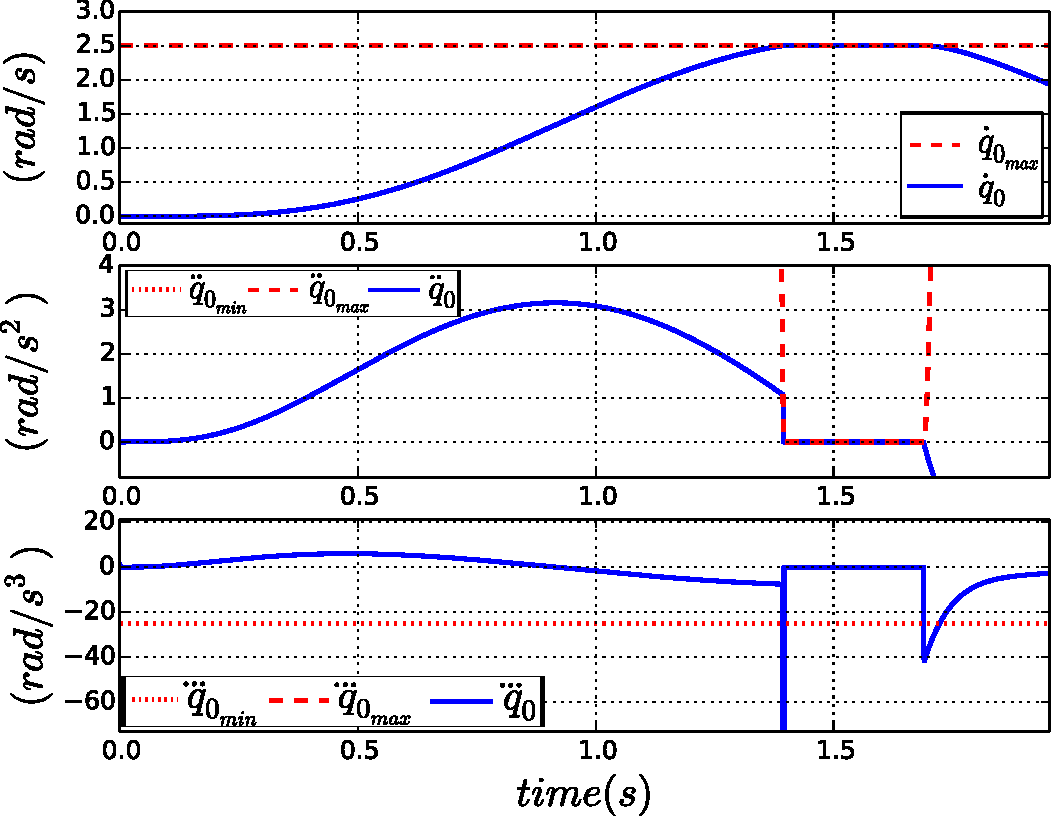
\includegraphics[width=1.0\columnwidth]{figures/0_Vel_constr_classic}}
\caption{Vel constr classic} 
\label{fig:0_Vel_constr_classic}
\end{figure}
%1
\begin{figure}[!htbp]
\centering
{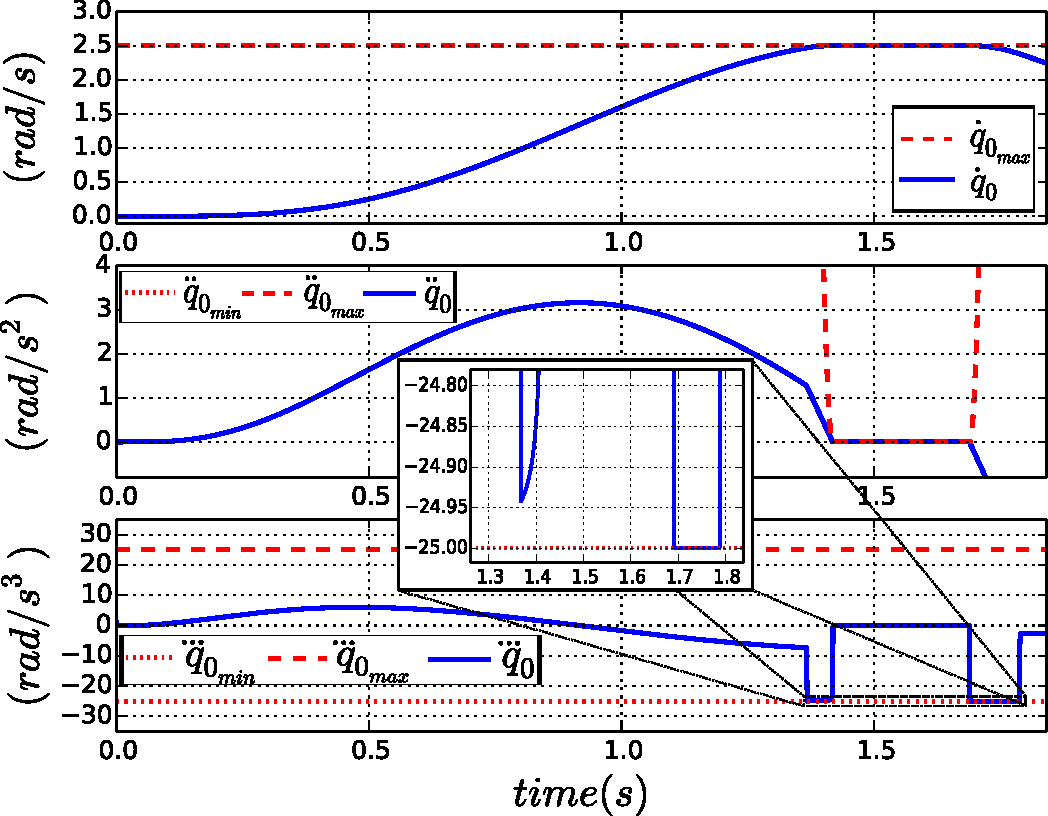
\includegraphics[width=1.0\columnwidth]{figures/1_Vel_constr_jerk_comp}}
\caption{Vel constr jerk comp} 
\label{fig:1_Vel_constr_jerk_comp}
\end{figure}
%4
\begin{figure}[!htbp]
\centering
{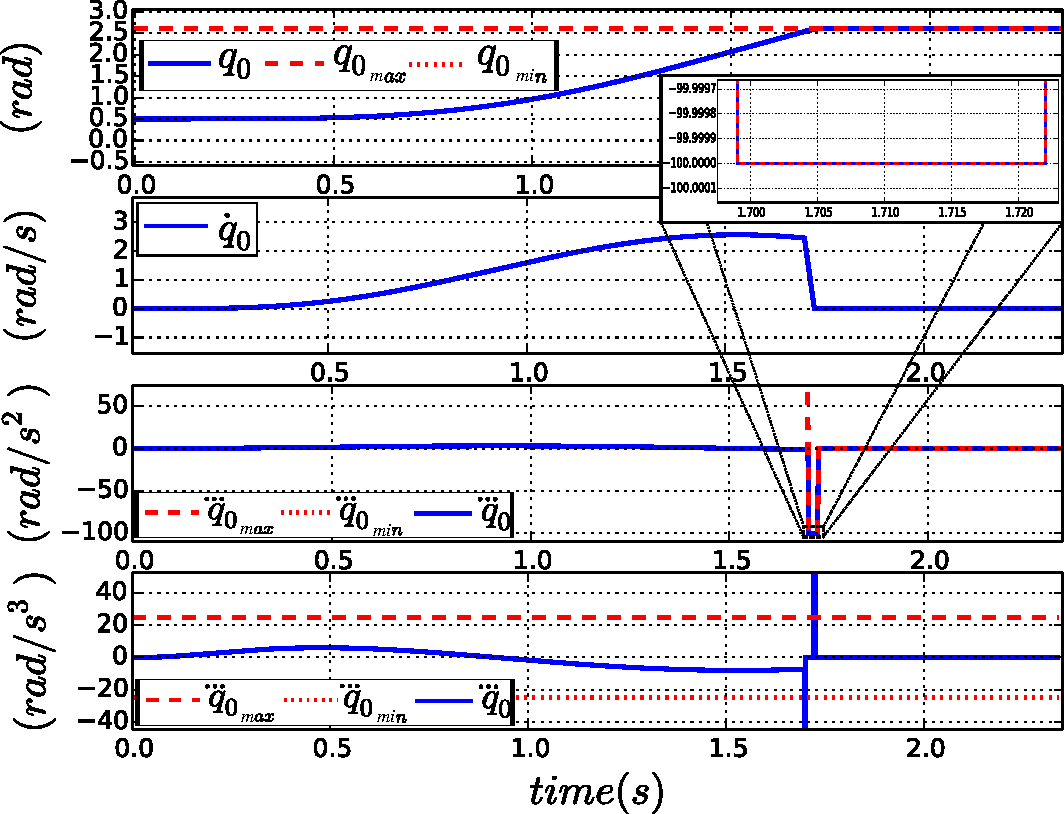
\includegraphics[width=1.0\columnwidth]{figures/4_Posi_constr_acc_comp_100}}
\caption{Posi constr acc comp 100} 
\label{fig:4_Posi_constr_acc_comp_100}
\end{figure}
%5
\begin{figure}[!htbp]
\centering
{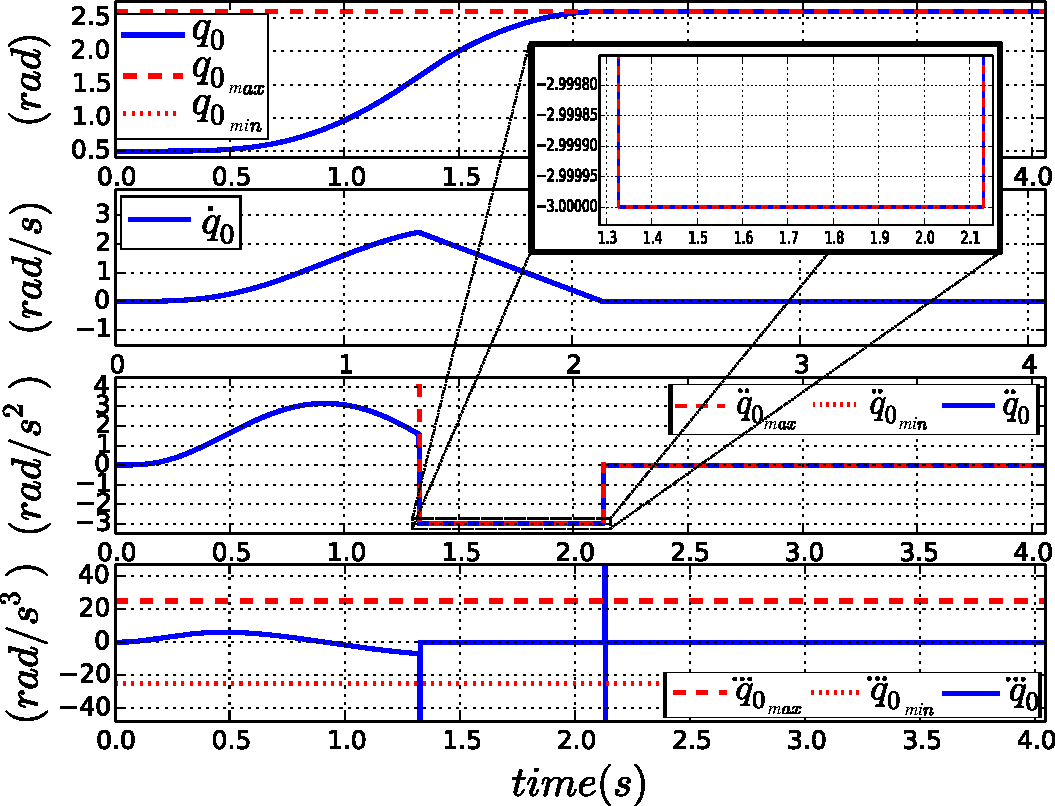
\includegraphics[width=1.0\columnwidth]{figures/5_Posi_constr_acc_comp_3}}
\caption{Posi constr acc comp 3} 
\label{fig:5_Posi_constr_acc_comp_3}
\end{figure}
%6
\begin{figure}[!htbp]
\centering
{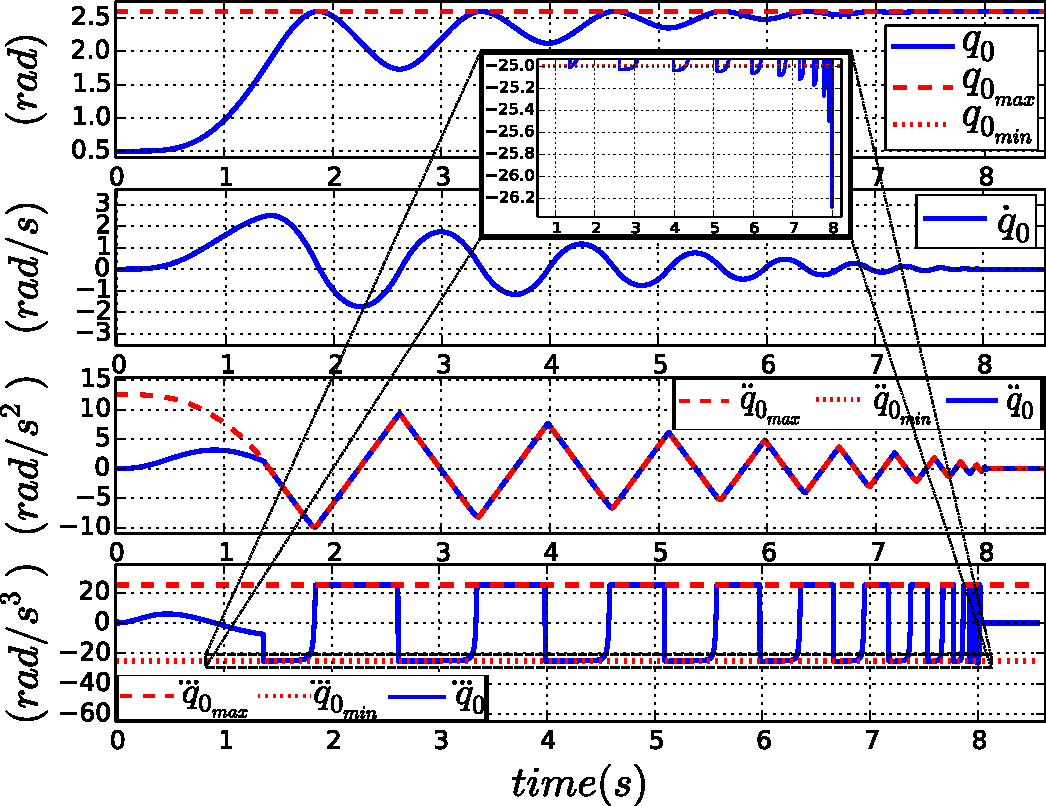
\includegraphics[width=1.0\columnwidth]{figures/6_Posi_constr_jerk_comp_25_non_complete_formula_backklash}}
\caption{Posi constr jerk comp 25 non complete formula backklash} 
\label{fig:6_Posi_constr_jerk_comp_25_non_complete_formula_backklash}
\end{figure}
%7
\begin{figure}[!htbp]
\centering
{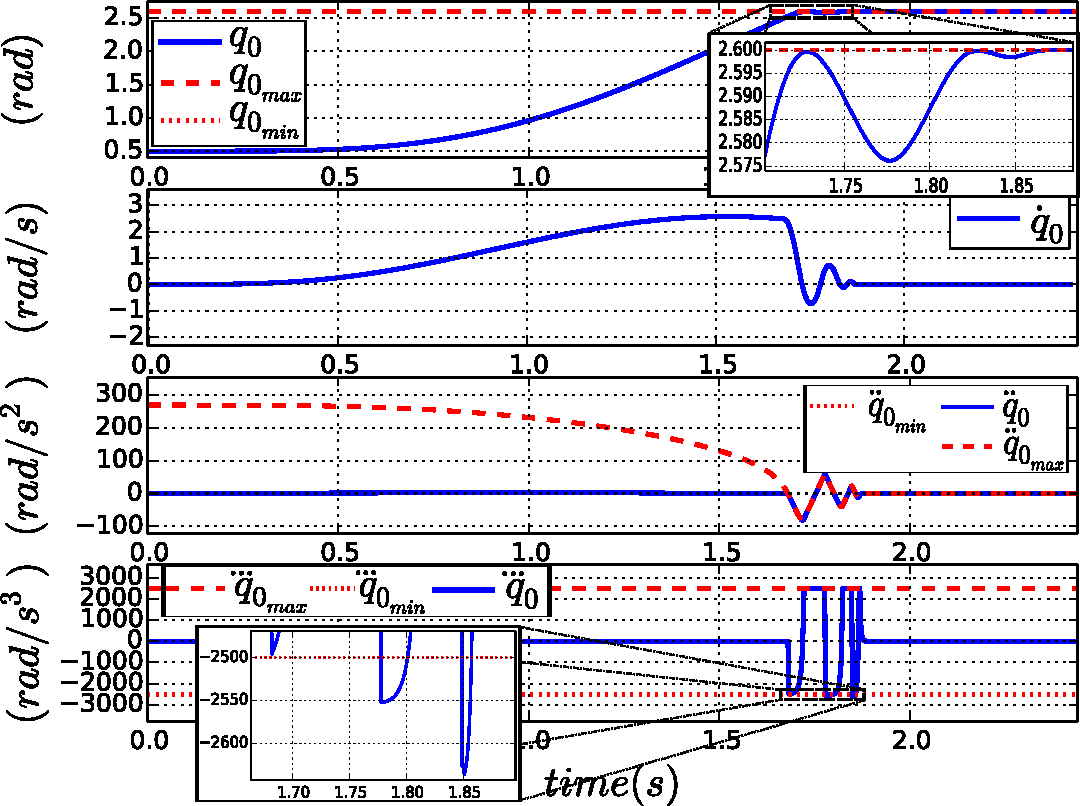
\includegraphics[width=1.0\columnwidth]{figures/7_Posi_constr_jerk_comp_2500_non_complete_formula_backklash}}
\caption{Posi constr jerk comp 2500 non complete formula backklash} 
\label{fig:7_Posi_constr_jerk_comp_2500_non_complete_formula_backklash}
\end{figure}
%8
\begin{figure}[!htbp]
\centering
{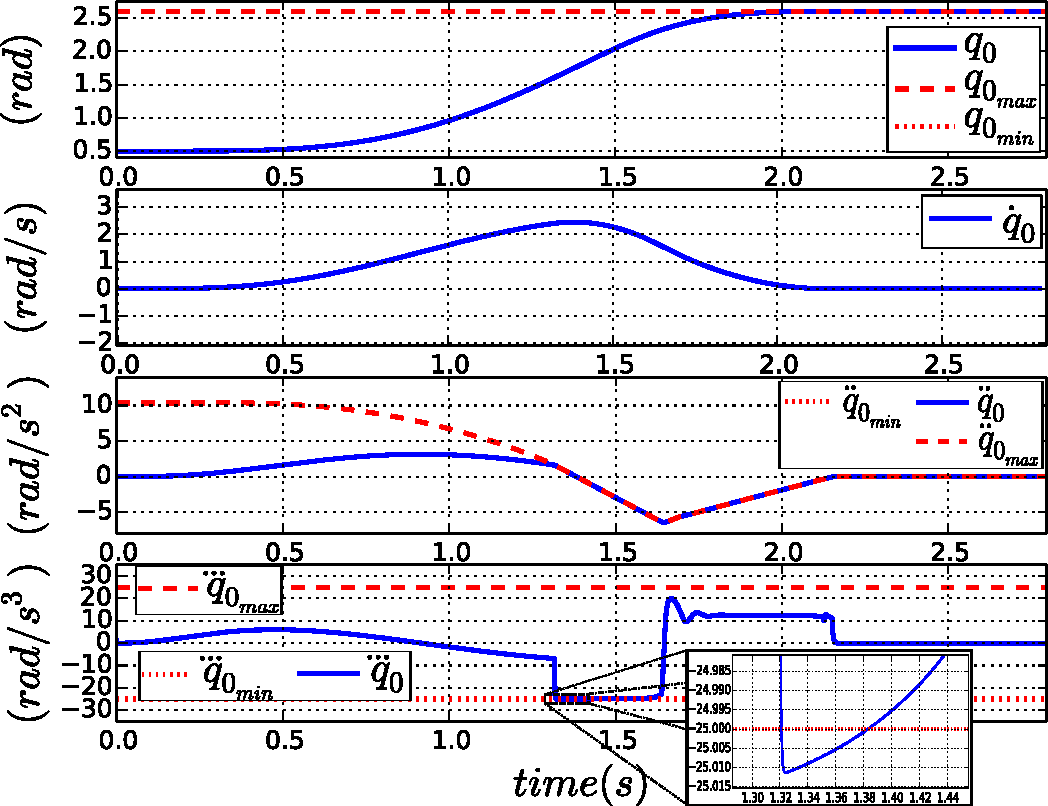
\includegraphics[width=1.0\columnwidth]{figures/8_Posi_constr_jerk_comp_25_complete_formula_no_backklash}}
\caption{Posi constr jerk comp 25 complete formula no backklash} 
\label{fig:8_Posi_constr_jerk_comp_25_complete_formula_no_backklash}
\end{figure}
%9
\begin{figure}[!htbp]
\centering
{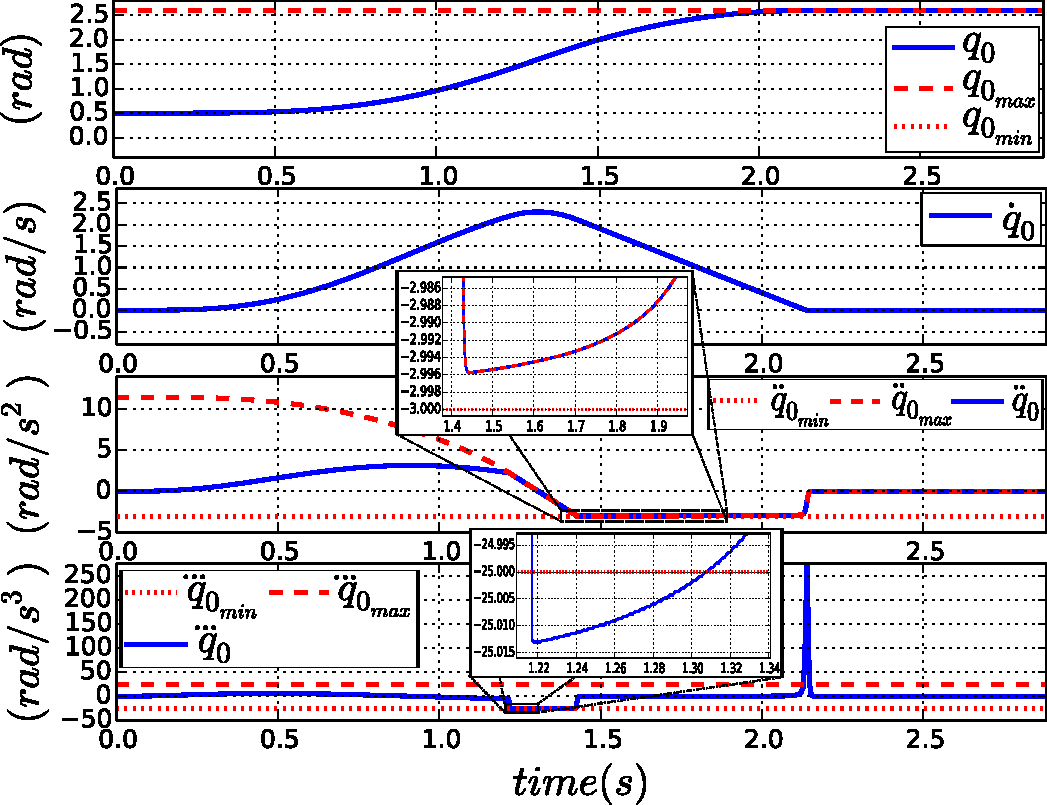
\includegraphics[width=1.0\columnwidth]{figures/9_Posi_constr_jerk_acc_comp_non_complete_formula_3}}
\caption{Posi constr jerk acc comp non complete formula 3} 
\label{fig:9_Posi_constr_jerk_acc_comp_non_complete_formula_3}
\end{figure}
%10
\begin{figure}[!htbp]
\centering
{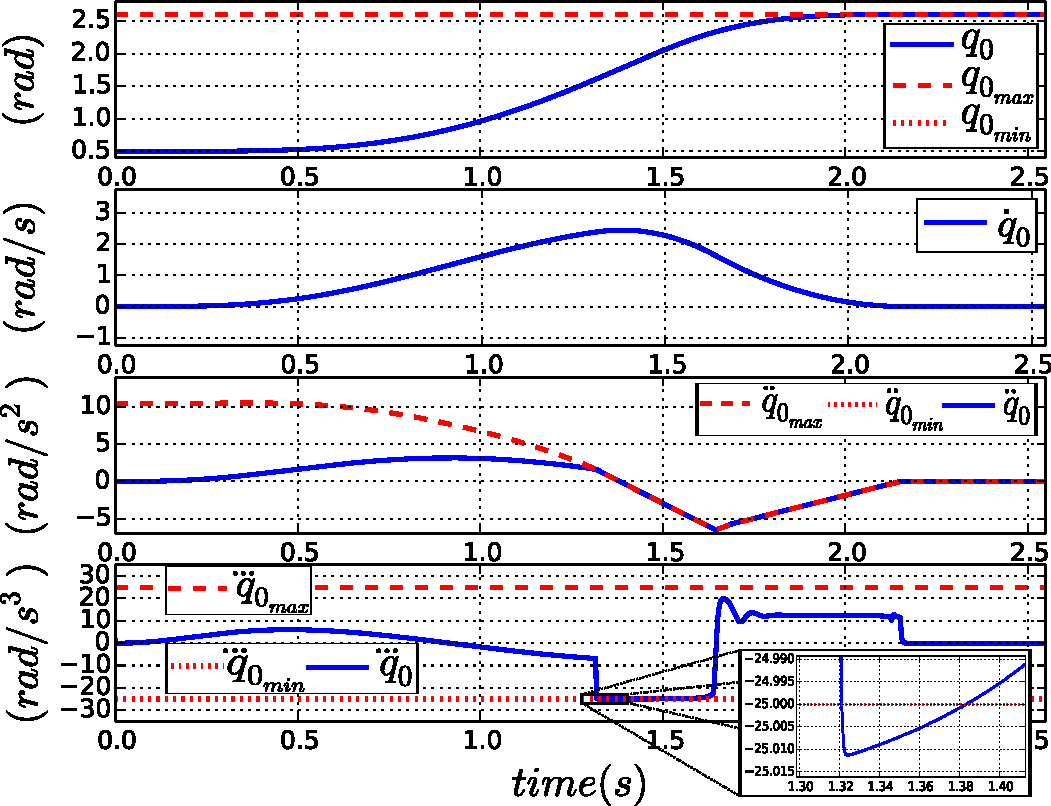
\includegraphics[width=1.0\columnwidth]{figures/10_Posi_constr_jerk_acc_comp_complete_formula_100}}
\caption{Posi constr jerk acc comp complete formula 100} 
\label{fig:10_Posi_constr_jerk_acc_comp_complete_formula_100}
\end{figure}
%11
\begin{figure}[!htbp]
\centering
{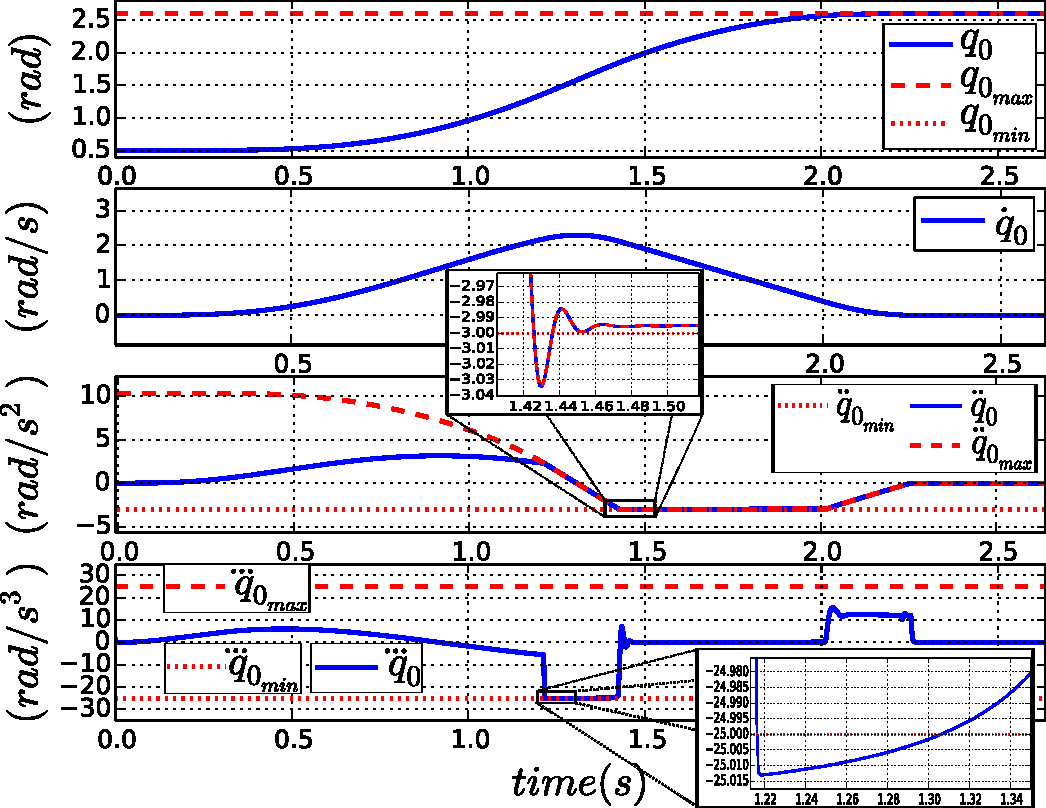
\includegraphics[width=1.0\columnwidth]{figures/11_Posi_constr_jerk_acc_comp_complete_formula_3}}
\caption{Posi constr jerk acc comp complete formula 3} 
\label{fig:11_Posi_constr_jerk_acc_comp_complete_formula_3}
\end{figure}

\newpage

%\subsection{Joint velocity constraint incompatibility with jerk limits (classic  \textit{Vs} new formulation)}
%For the first test, 
%
%\subsection{Joint position constraint incompatibility with decelera-
%tion limits (classic  \textit{Vs} new formulation)}
%
%\subsection{Joint position constraint incompatibility with jerk lim-
%its
% (classic  \textit{Vs} new formulation)}
%
%\subsection{Joint position constraint with both acceleration and
%jerk limits
% (classic  \textit{Vs} new formulation)}
%
%\subsection{Full constraints (classic  \textit{Vs} new formulation)}
%\\
%\\
%\\
%\\
\begin{figure}
\centering
{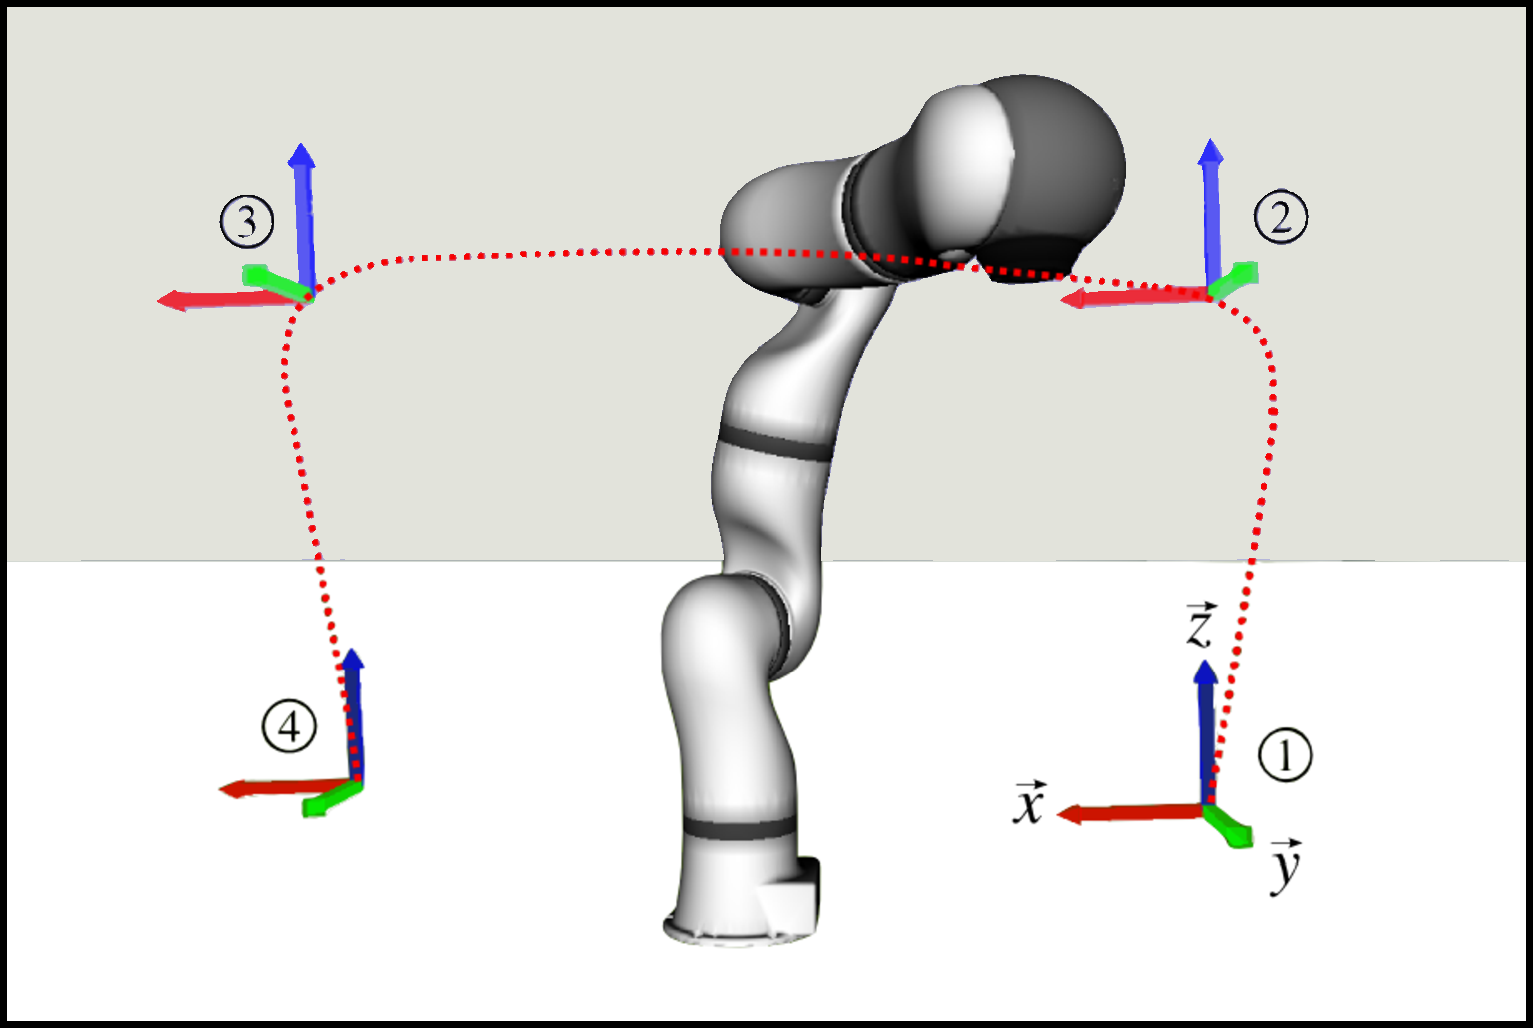
\includegraphics[width=1.0\columnwidth]{figures/kuka_in_xde_VOID}}
\caption{Kuka LWR4 serial robot within the XDE simulator. In red dots, the trajectory of the end-effector.} 
\label{fig:kuka_in_xde_VOID}
\end{figure}

%The controller described by (\ref{eq:ctrl_pb}) is implemented with the linear constraints (\ref{eq:qddot_FINAL_CONSTR_1}) and (\ref{eq:qddot_FINAL_CONSTR_2}) on the physical limitations of the system. During the movement of the robot, maximum/minimum actuators positions and velocities are reached and the constraints activated.

%\begin{figure*}
%\centering
%{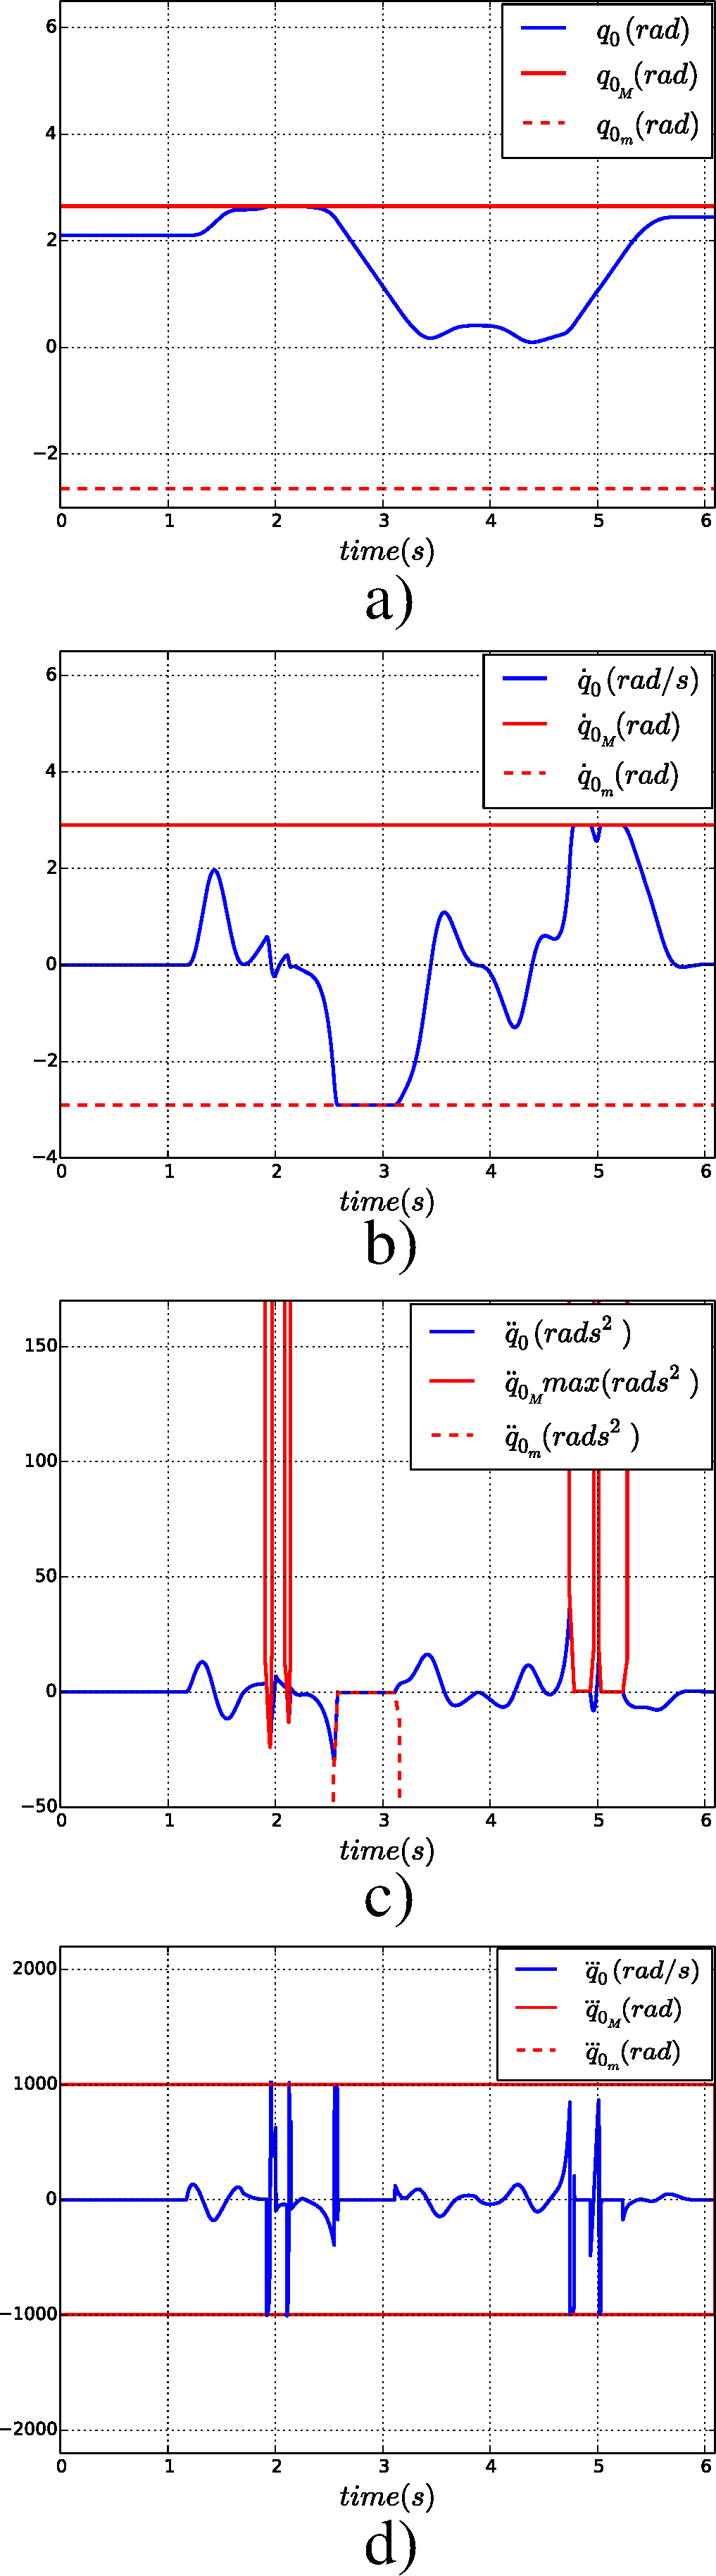
\includegraphics[width=0.8\columnwidth]{figures/q_qdot_qddot_qdddot}}
%\caption{a), b), c) and d) : Constrained articular position, velocity, acceleration and jerk of the first joint of the robot} 
%\label{fig:q_qdot_qddot_qdddo}
%\end{figure*}
%
%\begin{figure}[h]
%\centering
%{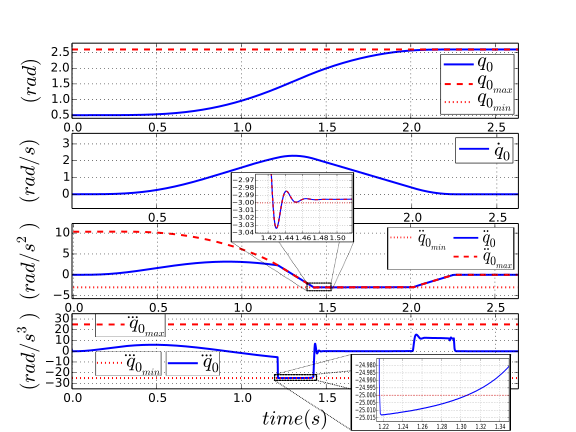
\includegraphics[width=1.0\columnwidth]{figures/comp_q,_q_ddot,_q_dddot_final_!!!}}
%\caption{comp_q,_q_ddot,_q_dddot_final_!!!.} 
%\label{fig:comp_q,_q_ddot,_q_dddot_final_!!!}
%\end{figure}

%\begin{figure}[h]
%\centering
%{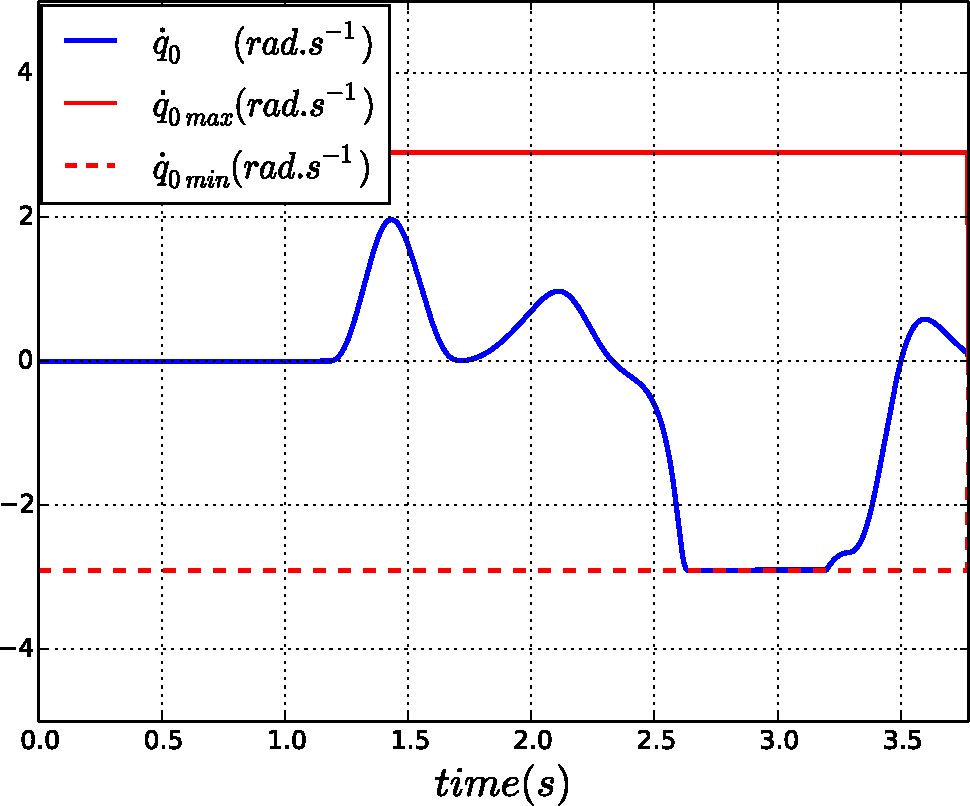
\includegraphics[width=0.9\columnwidth]{figures/1_q_dot_jerk_vel_constr}}
%\caption{$\dot{q}_{|k}, \dot{q}_{|k}_{_M0} and \dot{q}_{|k}_{_m0}$} 
%\label{fig:1_q_dot_jerk_vel_constr}
%\end{figure}
%
%\begin{figure}[h]
%\centering
%{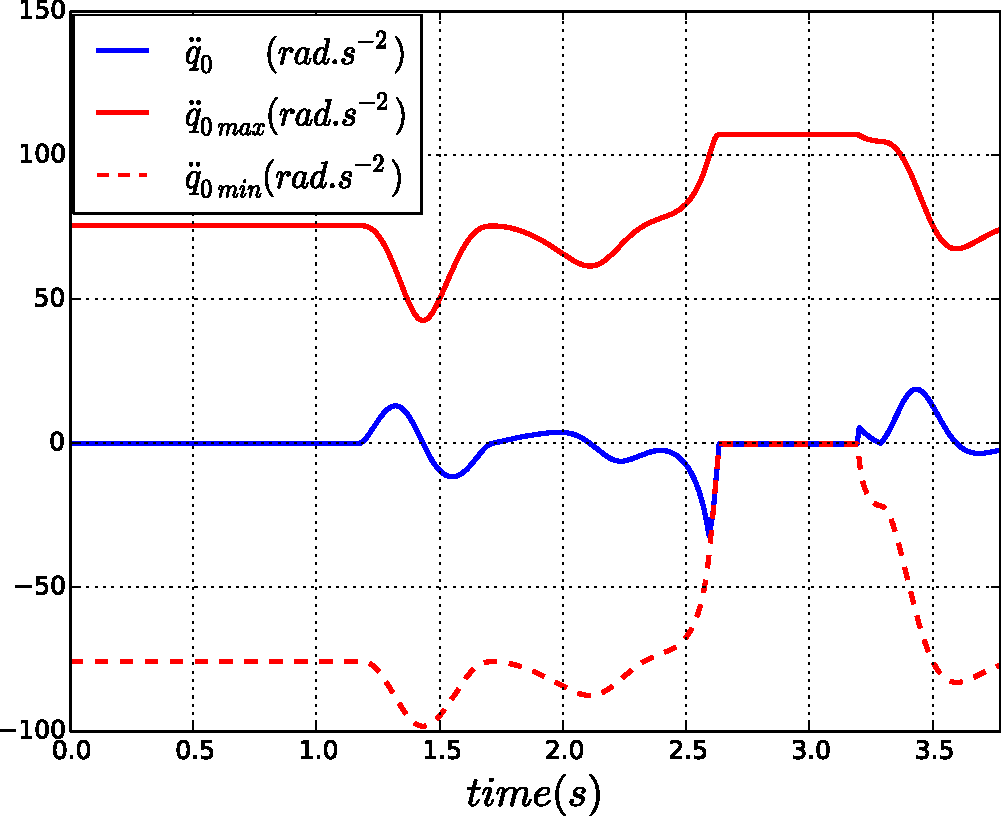
\includegraphics[width=0.93\columnwidth]{figures/2_q_dot_dot_jerk_vel_constr}}
%\caption{$\ddot{q}_{|k}, \ddot{q}_{|k}_{_M0} and \ddot{q}_{|k}_{_m0}$} 
%\label{fig:2_q_dot_dot_jerk_vel_constr}
%\end{figure}
%
%\begin{figure}[h]
%\centering
%{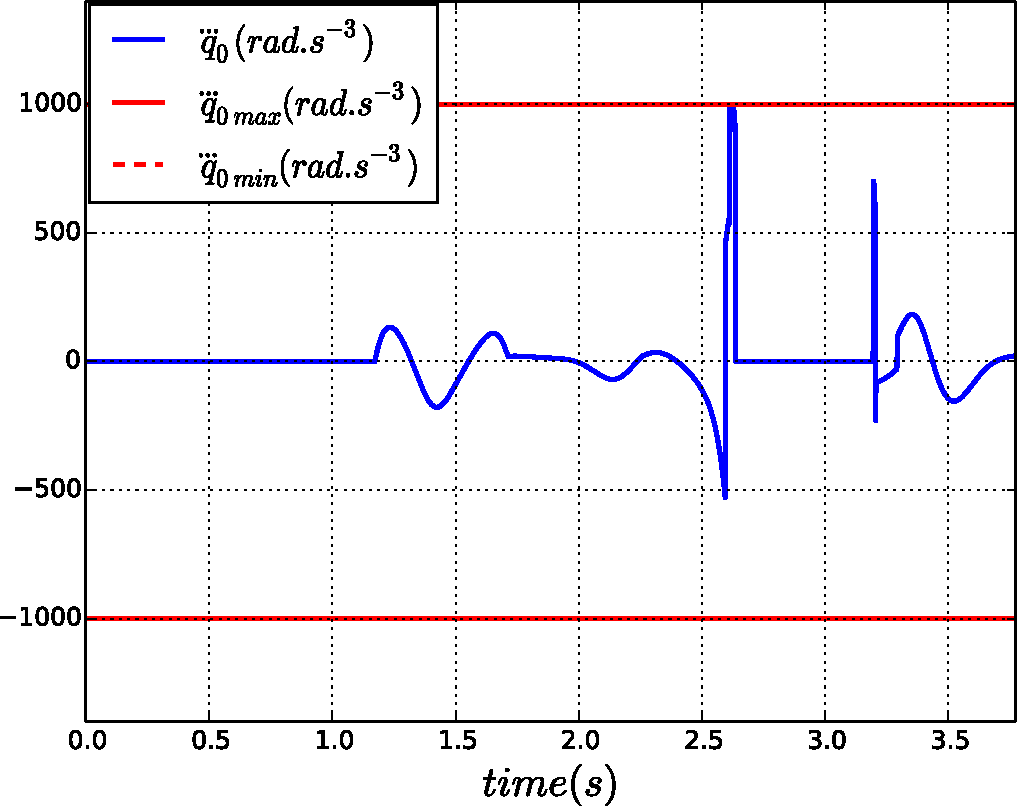
\includegraphics[width=0.93\columnwidth]{figures/3_q_dot_dot_dot_jerk_vel_constr}}
%\caption{$\dddot{q}_{|k}, \dddot{q}_{|k}_{_M0} and \dddot{q}_{|k}_{_m0}$} 
%\label{fig:3_q_dot_dot_dot_jerk_vel_constr}
%\end{figure}
%
%
%\begin{figure}[h]
%\centering
%{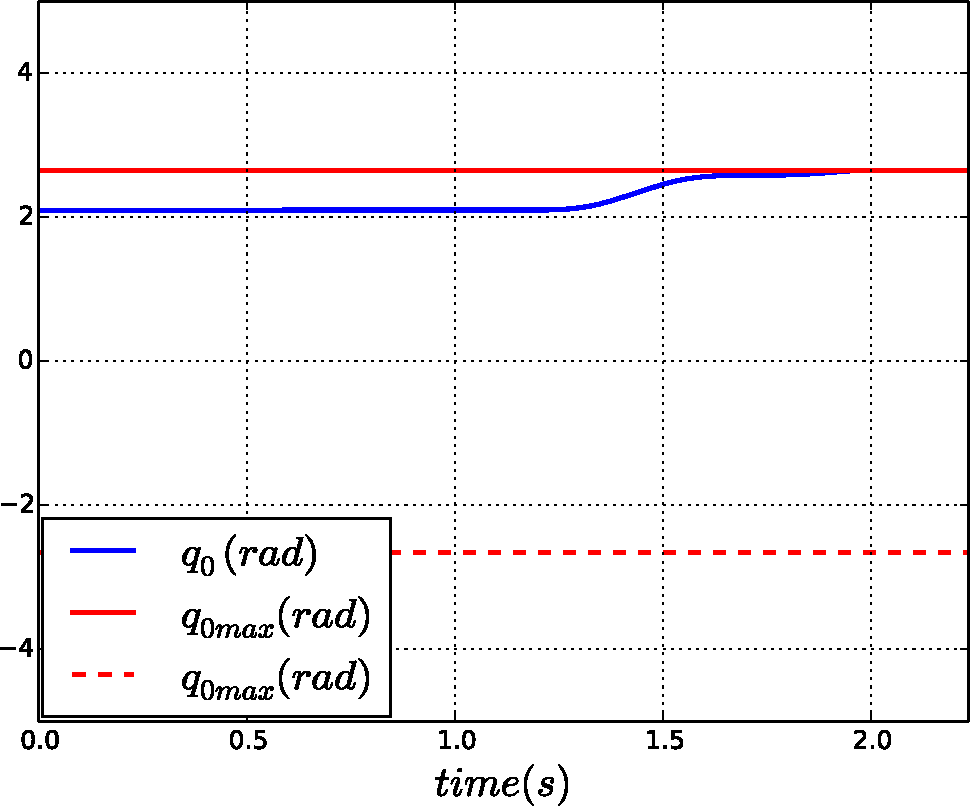
\includegraphics[width=0.9\columnwidth]{figures/4_q_acc_jerk_vel_constr}}
%\caption{$q_{|k}, q_{|k}_{_M0} and q_{|k}_{_m0}$} 
%\label{fig:4_q_acc_jerk_vel_constr}
%\end{figure}
%
%
%\begin{figure}[h]
%\centering
%{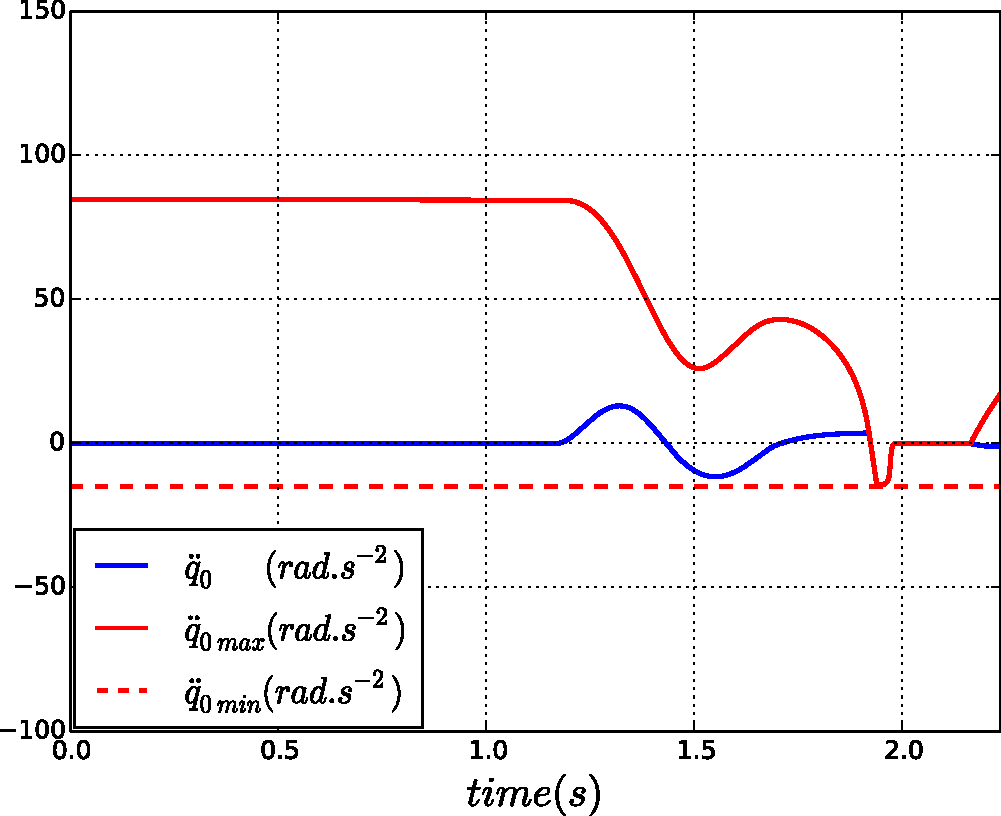
\includegraphics[width=0.9\columnwidth]{figures/5_q_dot_dot_acc_jerk_vel_constr}}
%\caption{$\ddot{q}_{|k}, \ddot{q}_{|k}_{_M0} and \ddot{q}_{|k}_{_m0}$} 
%\label{fig:5_q_dot_dot_acc_jerk_vel_constr}
%\end{figure}
%
%
%
%\begin{figure}[h]
%\centering
%{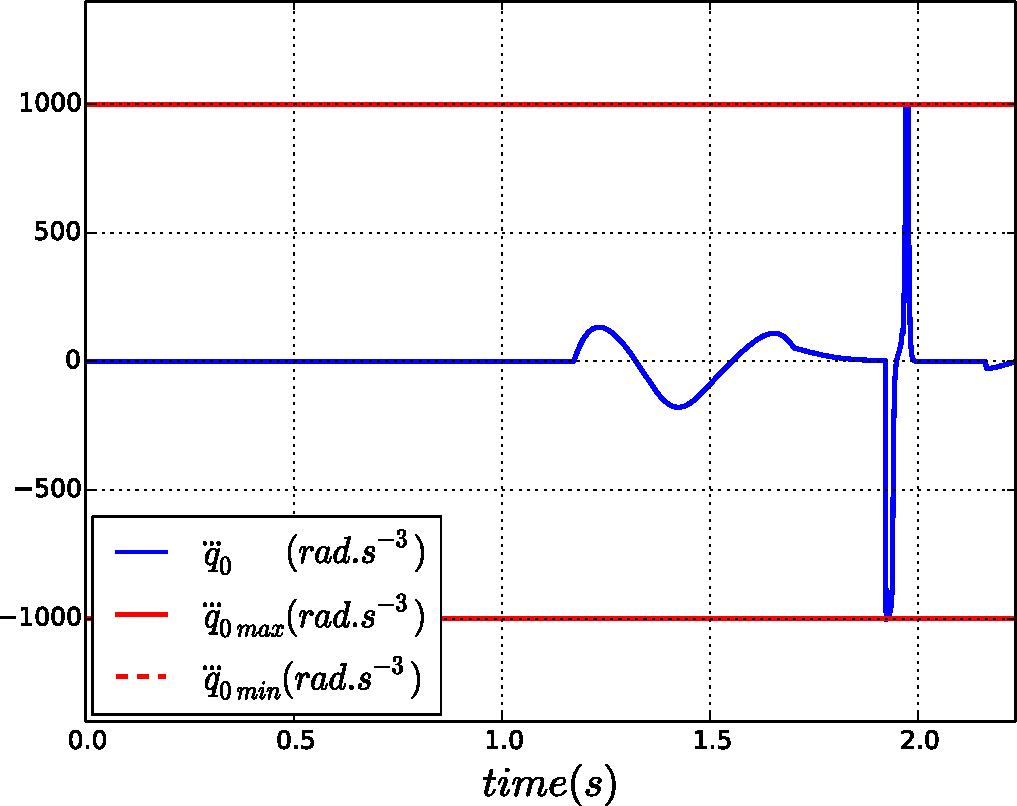
\includegraphics[width=0.93\columnwidth]{figures/6_q_dot_dot_dot_acc_jerk_vel_constr}}
%\caption{$\dddot{q}_{|k}, \dddot{q}_{|k}_{_M0} and \dddot{q}_{|k}_{_m0}$} 
%\label{fig:6_q_dot_dot_dot_acc_jerk_vel_constr}
%\end{figure}


%From Fig.~\ref{fig:q_qdot_qddot_qdddo} we can see that all the actuators limitations : $\vect{q}_{m}, \vect{q}_{M}, \vect{\dot{q}}_{m}, \vect{\dot{q}}_{M}, \vect{\ddot{q}}_{m}, \vect{\ddot{q}}_{M}, \vect{\dddot{q}}_{m}$ and $\vect{\dddot{q}}_{M}$ are respected. $\vect{\dddot{q}}_{M}, \vect{\dddot{q}}_{m}$ are respectively chosen $+1000$ and $-1000 (rad/s^3)$ with a control time step of $1 ms$.
%
%
%\section{Conclusion}
%\label{sec:constrcompconclusion}
%The presented work allows a robotic system to be able to cope with static constraints without violating its reaction capabilities. An application on the articular velocity and position limits of a KUKA LWR4 is performed. Within the producible values of torque and jerk, the optimization control algorithm is capable of delivering an optimal solution every time step. Dynamic constraints however still need to be expressed and solved considering the same approach. 


\newpage


\section{Appendix - Proof for the mathematical reformulation of the articular position and velocity constraints}


\subsection{Computation of deceleration capabilities ($\boldsymbol{\ddot{q}}_m$ and $\boldsymbol{\ddot{q}}_M$)}
$\boldsymbol{\ddot{q}}_m$, $\boldsymbol{\ddot{q}}_M$ are computed from the maximum $\vect{\tau}_M$ and minimum $\vect{\tau}_m$ torques producible by the actuators :

\begin{gather}
\argmin \limits_{\boldsymbol{\tau}} \boldsymbol{M}(\vect{q})^{-1} (\vect{\tau}-\vect{b}(\vect{q},\vect{\dot{q}})),
\raisetag{-.5em}
\label{eq:qddot_minimizing_opt_1}
\end{gather}

\begin{gather}
\argmax \limits_{\boldsymbol{\tau}} \boldsymbol{M}(\vect{q})^{-1} (\vect{\tau}-\vect{b}(\vect{q},\vect{\dot{q}})),
\raisetag{-.5em}
\label{eq:qddot_maximizing_opt_2}
\end{gather}

s.t: $\vect{\tau}_m \leq \vect{\tau} \leq \vect{\tau}_M$

Whith : 

\begin{equation}
\vect{\ddot{q}}_m =  \boldsymbol{M}(\vect{q})^{-1} (\vect{\tau}_{min}-\vect{b}(\vect{q},\vect{\dot{q}})), 
\label{eq:qddot_minimizing}
\end{equation}

\begin{equation}
\vect{\ddot{q}}_M =  \boldsymbol{M}(\vect{q})^{-1} (\vect{\tau}_{max}-\vect{b}(\vect{q},\vect{\dot{q}})), 
\label{eq:qddot_maximizing}
\end{equation}

$\vect{\tau}_{min}$ and $\vect{\tau}_{max}$ are respectively the solutions of (\ref{eq:qddot_minimizing_opt_1}) and (\ref{eq:qddot_maximizing_opt_2}). 



\subsection{Dynamic and kinematic control input parameters relationship}
Analogue to (\ref{eq:cmd_input_dyn}), in case the robot is controlled at the kinematic level , for a velocity control input $\vect{\dot{q}}_{|k}^{c}$ computed at the current time-step $k$, the expected articular velocity at the next time-step $k+1$ is : 
\begin{equation} 
\vect{\dot{q}}_{|k+1} =\vect{\dot{q}}_{|k}^{c} 
\label{eq:cmd_input_kin}
\end{equation}
At the dynamic level, the articular velocity at the next time-step for a $\vect{\ddot{q}}_{|k}^{c}$ acceleration control input is expressed : 
\begin{equation} 
\vect{\dot{q}}_{|k+1}=\vect{\dot{q}}_{|k}+\vect{\ddot{q}}_{|k}^{c} \delta t
\label{eq:cmd_input_dyn2}
\end{equation}
Therefore, for a robot to produce the same movement at both control levels, the relationship between the two control inputs is expressed : 
\begin{equation} 
\vect{\dot{q}}_{|k}^{c}=\vect{\dot{q}}_{|k}+\vect{\ddot{q}}_{|k}^{c} \delta t
\label{eq:kin_dyn_ctrl_inp_rela}
\end{equation}
Finally, a constraint on $\vect{\dot{q}}_{|k}^{c}$ can easily be reflected on $\vect{\ddot{q}}_{|k}^{c}$.



Let $q_{|k}, \dot{q}_{|k}, \ddot{q}_{|k}$ and $\dddot{q}_{|k}$ be the sequences of joint positions, velocities, accelerations and jerk. In discrete time, the motion is modelized by : 

\begin{equation} 
\left\{\begin{array}{lcl}
\vect{q}_{|k+1} = \vect{q}_{|k} + \vect{\dot{q}}_{|k} \delta t, \\
\vect{\dot{q}}_{|k+1} = \vect{\dot{q}}_{|k} + \vect{\ddot{q}}_{|k} \delta t, \\
\vect{\ddot{q}}_{|k+1} = \vect{\ddot{q}}_{|k} + \vect{\dddot{q}}_{|k} \delta t.
\end{array}\right.
\label{eq:discretized_dynamics}
\end{equation}

\subsection{Joint jerk and velocity limits}


If we suppose $\dot{q}_{|k} > 0$ and $\dddot{q}_m < 0$ (negative jerk example), the condition $\dot{q}(k+n_1) \leq \dot{q}_M$ for all integer $n_1$ leads to :

\begin{equation}
\begin{split}
\ddot{q}_{|k} \leq \frac{\dot{q}_M-\dot{q}_{|k}}{n_1 \delta t} - \frac{(n_1-1)}{2} \dddot{q}_m \delta t 
\label{eq:q_ddot_vel_jerk_comp}
\end{split}
\end{equation}

Where $n_1$, the integer minimizing the right hand side of (\ref{eq:q_ddot_vel_jerk_comp}). By diferentiating this expression w.r.t $n_1$ :

\begin{equation} 
\left. \begin{array}{r} 
n_1 \geq 1 \\
\frac{-(\dot{q}_M-\dot{q}_{|k})}{n_1^2 \delta t} - \frac{1}{2} \dddot{q}_m \delta t = 0
\end{array} \right\} 
\Leftrightarrow n_1=-\frac{\sqrt{-2\dddot{q}_m(\dot{q}_M-\dot{q}_{|k})}}{\dddot{q}_m \delta t}
\label{eq:n_1_eq}
\end{equation}

$n_1$ must be $\geq 1$ so the acceleration constraint is not violated. Moreover, the presented method may fail in case of any measurements errors. 

With : $q_{|k+1} = q_{|k}+\dot{q}_{|k} \delta t$, an overestimation \footnote{ Because it is computed during a braking phase, the estimation of the position for the next time step will always be less than the real position : $q_{estimated}_{|k+1} \leq q_{real}_{|k+1}$} of the actuator position at the next time step.

$n_3$ is the integer minimizing the right hand side of (\ref{eq:q_dot_posi_acc_comp}). By differentiating this expression w.r.t $n_3$ :

\begin{equation} 
\left. \begin{array}{r} 
n_3 \geq 1 \\
\frac{-(q_M-q_{|k})}{n_3^2 \delta t} - \frac{1}{2} \ddot{q}_m \delta t= 0
\end{array} \right\} 
\Leftrightarrow n_3=-\frac{\sqrt{-2\ddot{q}_m(q_M-q_{|k})}}{\ddot{q}_m \delta t}
\label{eq:n_3_eq}
\end{equation}

\subsection{Joint jerk and position limits}
In case of constant jerk $\dddot{q}_m$, the position evolution in $n_5$ 

If we suppose $\dot{q}_{|k} > 0$ and $\dddot{q}_m < 0$ (negative jerk example), the condition $q(k+n_5) \leq q_M$ for all integer $n_5$ leads to : 

\begin{equation}
\begin{split}
\ddot{q}_{|k} \leq \frac{2(q_M-q_{|k})}{(n_5^2-n_5) \delta t^2} - \frac{2 \dot{q}_{|k}}{(n_5-1) \delta t} - \frac{(\frac{n_5^2}{3}-n_5+\frac{2}{3})\ddot{q}_m \delta t}{(n_5-1)} 
\label{eq:q_ddot_posi_jerk_comp}
\end{split}
\end{equation}

$n_5$ is the integer minimizing the right hand side of (\ref{eq:q_ddot_posi_jerk_comp}). By differentiating this expression w.r.t $n_5$ :

\begin{equation}
\left\{\begin{array}{lcl}
n_5 \geq 3 \\
\begin{split}
-&(\frac{1}{3} \dddot{q}_m_{|k} \delta t^3) n_5^4 + (\frac{2}{3} \ddot{q}_{|k} \delta t^3) n_5^3  \\
+&(2 \dot{q}_{|k} \delta t - \frac{1}{3} \dddot{q}_m_{|k} \delta t^3) n_5^2 \\
+&(4 (q_M-q_{|k}) n_5 - 2(q_M-q_{|k}=0
\end{split}
\end{array}\right.
\label{eq:n_5_eq}
\end{equation}

Indeed, $n_5$ must be $\geq 3$ so $\dddot{q}_m$ is always part of (\ref{eq:q_ddot_posi_jerk_comp}). 

\subsection{Joint jerk, acceleration and position limits}
To avoid violating the position constraint, the braking movement is usually induced as following : first start jerking with maximum jerk in the opposite direction until maximum deceleration capabilities are reached; Then bring both jerk and deceleration to zero (see Fig.~3.3). Therefore, both $\ddot{q}_m$, $\ddot{q}_M$ and $\dddot{q}_m$, $\dddot{q}_M$  
should appear in the position constraint formulation. In the case of a braking phase as just described, the position evolution in $n_7+n_9$ iterations:
%\footnote{$n_7$ and $n_9$ are respectively: the number of iterations corresponding to a braking movement with negative jerk independently from the acceleration/deceleration capabilities and the number of iterations corresponding to the same braking movement with a deceleration.}

\begin{equation}
\begin{split}
q(k+n_7+n_9)=q(k+n_7) + n_9 \dot{q}(k+n_7) \delta t  + \frac{(n_9^2-n_9)}{2} \ddot{q}_m \delta t^2
\label{eq:q_evolution_with_const_qddot_m_and_qdddot_m_1}
\end{split}
\end{equation} 

With : $q(k+n_7)$ equivalent to (\ref{eq:q_evolution_with_const_qdddot_m}) and $\dot{q}(k+n_7)$ to (\ref{eq:q_dot_evolution_with_const_qdddot_m}).
(\ref{eq:q_evolution_with_const_qddot_m_and_qdddot_m_1}) becomes : 

\begin{equation}
\begin{split}
q(k+n_7+n_9) & =q_{|k} + (n_7+n_9) \dot{q}_{|k} \delta t + [\frac{(n_7^2-n_7)}{2}+n_7 n_9] \ddot{q}_{|k} \delta t^2 \\
             & + [\frac{n_7^3}{6}-\frac{n_7^2}{2}+\frac{n_7}{3}+\frac{n_9(n_7^2-n_7)}  {2}] \dddot{q}_m \delta t^3 + \frac{(n_9^2-n_9)}{2} \ddot{q}_m \delta t^2
\label{eq:q_evolution_with_const_qddot_m_and_qdddot_m_2}
\end{split}
\end{equation} 

If we suppose $\dot{q}_{|k} > 0$ with $\ddot{q}_m < 0$ and $\dddot{q}_m < 0$ (deceleration and negative jerk example), the condition $q(k+n_7+n_9) \leq q_M$ for all integers $n_7$ and $n_9$ leads to :

\begin{equation}
\begin{split}
\ddot{q}_{|k} & \leq \frac{(q_M - q_{|k})}{(\frac{n_7^2 - n_7}{2} + n_7 n_9)\delta t^2}-\frac{[\frac{n_7^3}{6} - \frac{n_7^2}{2} + \frac{n_7}{3} + \frac{n_9(n_7^2-n_7)}{2}]}{(\frac{n_7^2 - n_7}{2} + n_7 n_9)} \dddot{q}_m \delta t \\ & - \frac{(n_9^2-n_9)}{(n_7^2 - n_7 + 2 n_7 n_9)}  \ddot{q}_m- \frac{(n_7+n_9)}{(\frac{n_7^2 - n_7}{2} + n_7 n_9) \delta t} \dot{q}_{|k}
\label{eq:Constr_comp_posi_acc_jerk_1_appendix}
\end{split}
\end{equation}

If the control performed at the kinematic level : 

\begin{equation}
\begin{split}
\dot{q}_{|k} & \leq \frac{(q_M - q_{|k})}{(n_7 + n_9) \delta t}  -\frac{[\frac{(n_7^2-n_7)}{2} + n_7 n_9]}{(n_7 + n_9)}  \ddot{q}_{|k} \delta t\\ 
           & - \frac{[\frac{(n_7^3)}{6} + \frac{(n_7^2)}{2} + \frac{(n_7)}{3} + \frac{n_9 (n_7^2 - n_7)}{2}]}{(n_7 + n_9)} \dddot{q}_m \delta t^2 - \frac{(n_9^2-n_9)}{2(n_7 + n_9)} \ddot{q}_m \delta t
\label{eq:Constr_comp_posi_acc_jerk_1_kinema_appendix}
\end{split}
\end{equation}

$n_7$ and $n_9$ minimize the right hand side of (\ref{eq:Constr_comp_posi_acc_jerk_1_appendix}). These two integers are computed numerically. Knowing that the braking phase lasts only for a limited amount of time steps. All the combinations $(n_7, n_9)$ with : $1\leq n_7 \leq500$ and $3 \leq n_9 \leq 100$ are to be tried. The maximum/minimum values of $n_7$ and $n_9$ to be tested are for now fixed heuristically. 





\bibliographystyle{IEEEtran}
\bibliography{IEEEabrv,IROS_PAPER_Vincent_V2}


\end{document}
